\documentclass[11pt]{extbook}

\usepackage{geometry}

\usepackage{fancyvrb}
\usepackage{color}
\usepackage{graphicx}
\usepackage{fullpage}
\usepackage{verbatim}
\usepackage{tikz}
\usepackage{listings}
\usepackage[yyyymmdd,hhmmss]{datetime}
\usepackage{rotating}
\usepackage{authblk}
\usepackage{amsfonts}
\usepackage{amsmath}
\usepackage{amssymb}
\usepackage{todonotes}
\usepackage{titlesec}
\usepackage[mathlines]{lineno}
\usepackage{tabularx}
\usepackage{enumitem}
\usepackage{bm}
\usepackage{etoolbox}
\usepackage{pdflscape}
\usepackage{threeparttable}
\usepackage{hyperref}
\usepackage{multirow}
\usepackage{graphicx}

%TGM:  Added these packages to fix underscore rendering
\usepackage{lmodern} 
\usepackage[T1]{fontenc}

\setcounter{secnumdepth}{3}
\setcounter{tocdepth}{3}

\titleformat{\paragraph}
{\normalfont\normalsize\bfseries}{\theparagraph}{1em}{}
\titlespacing*{\paragraph}
{0pt}{3.25ex plus 1ex minus .2ex}{1.5ex plus .2ex}

\newtoggle{assign}
\toggletrue{assign}

\newcommand{\qg}{\u{g}}
\newcommand{\qG}{\u{G}}
\newcommand{\qc}{\c{c} }
\newcommand{\qC}{\c{C}}
\newcommand{\qs}{\c{s}}
\newcommand{\qS}{\c{S}}
\newcommand{\qu}{\"{u}}
\newcommand{\qU}{\"{U}}
\newcommand{\qo}{\"{o}}
\newcommand{\qO}{\"{O}}
\newcommand{\qI}{\.{I}}
\newcommand{\wa}{\^{a}}
\newcommand{\wA}{\^{A}}

\begin{document}

\linenumbers

\newcommand{\kron}{\mathbin{\text{\footnotesize \textcircled{\raisebox{-0.3pt}{\footnotesize $\otimes$}}}}}
\newcommand{\grbarray}[1]{\bm{#1}}
\newcommand{\scalar}[1]{{#1}}
\renewcommand{\vector}[1]{{\bf #1}}
\renewcommand{\matrix}[1]{{\bf #1}}
\renewcommand{\arg}[1]{{\sf #1}}
\newcommand{\zip}{{\mbox{zip}}}
\newcommand{\zap}{{\mbox{zap}}}
\newcommand{\ewiseadd}{{\mbox{\bf ewiseadd}}}
\newcommand{\ewisemult}{{\mbox{\bf ewisemult}}}
\newcommand{\mxm}{{\mbox{\bf mxm}}}
\newcommand{\vxm}{{\mbox{\bf vxm}}}
\newcommand{\mxv}{{\mbox{\bf mxv}}}
\newcommand{\gpit}[1]{{\sf #1}}
\newcommand{\ie}{{i.e.}}
\newcommand{\eg}{{e.g.}}
\newcommand{\nan}{{\sf NaN}}
\newcommand{\nil}{{\bf nil}}
\newcommand{\ifif}{{\bf if}}
\newcommand{\ifthen}{{\bf then}}
\newcommand{\ifelse}{{\bf else}}
\newcommand{\ifendif}{{\bf endif}}
\newcommand{\zero}{{\bf 0}}
\newcommand{\one}{{\bf 1}}
\newcommand{\true}{{\sf true}}
\newcommand{\false}{{\sf false}}
\newcommand{\syntax}{{Math Notation}}

\newcommand{\Dinn}{\mbox{$D_{in}$}}
\newcommand{\Din}[1]{\mbox{$D_{in_{#1}}$}}
\newcommand{\Dout}{\mbox{$D_{out}$}}

\newcommand{\bDinn}{\mbox{$\mathbf{D}_{in}$}}
\newcommand{\bDin}[1]{\mbox{$\mathbf{D}_{in_{#1}}$}}
\newcommand{\bDout}{\mbox{$\mathbf{D}_{out}$}}

\newcommand{\scott}[1]{{{\color{violet}[Scott: #1]}}}
\newcommand{\tim}[1]{{{\color{teal}[Tim: #1]}}}
\newcommand{\ben}[1]{{{\color{blue}[Ben: #1]}}}
\newcommand{\will}[1]{{{\color{red}[Will: #1]}}}

%\newcommand{\scott}[1]{}
%\newcommand{\tim}[1]{}
%\newcommand{\ben}[1]{}
%\newcommand{\will}[1]{}

\renewcommand{\comment}[1]{{}}
\newcommand{\glossBegin}{\begin{itemize}}
\newcommand{\glossItem}[1]{\item \emph{#1}: }
\newcommand{\glossEnd}{\end{itemize}}

\setlength{\parskip}{0.5\baselineskip}
\setlength{\parindent}{0ex}

%\usepackage{draftwatermark}
%\SetWatermarkText{DRAFT}
%\SetWatermarkScale{2}

\renewcommand{\thefootnote}{\fnsymbol{footnote}}
\setcounter{footnote}{1}


%-----------------------------------------------------------------------------
% From Gabor's Notation document
\newbool{colored}
\booltrue{colored}
%\IfFileExists{./colored}{\booltrue{colored}}{\boolfalse{colored}}
\newbool{ascii}
\boolfalse{ascii}
%\IfFileExists{./ascii}{\booltrue{ascii}}{\boolfalse{ascii}}

\newcommand{\grbm}[1]{{\ifbool{colored}{\color{brown}}{}{\mathbf{#1}}}}% matrix
\newcommand{\grbv}[1]{{\ifbool{colored}{\color{violet}}{}{\mathbf{#1}}}}% vector
\newcommand{\grba}[1]{{\ifbool{colored}{\color{gray}}{}{\mathit{#1}}}}% array
\newcommand{\grbs}[1]{{\ifbool{colored}{\color{blue}}{}{\mathit{#1}}}}% scalar

\newcommand{\grbstr}[1]{{s(#1)}}
\newcommand{\grbmask}[1]{\langle #1 \rangle}
\newcommand{\grbmaskreplace}[1]{\langle\!\langle #1 \rangle\!\rangle}
\newcommand{\grbneg}{\neg}

% use the \mapsfrom symbol extracted from the stix package as suggested in https://tex.stackexchange.com/a/331899/71109
%\DeclareFontEncoding{LS1}{}{}
%\DeclareFontSubstitution{LS1}{stix}{m}{n}
%\DeclareSymbolFont{arrows1}{LS1}{stixsf}{m}{n}
%\DeclareMathSymbol{\mapsfrom}{\mathrel}{arrows1}{"AB}

\newcommand{\mapsfrom}{\mathrel{\reflectbox{\ensuremath{\mapsto}}}}
\newcommand{\grbassign}{\mapsfrom}

\newcommand{\grbf}[2]{\grboperation{#1}{#2}}
\newcommand{\grbreduce}[4]{[ {#1}_{#2}\, #3(#4) ]}
\newcommand{\grbt}{^{\top}} % transpose
\newcommand{\grbdiv}{\grbbinaryop{\oslash}}
\newcommand{\grbminus}{\grbbinaryop{\ominus}}
\newcommand{\grbaccumeq}[1]{\mathbin{\ensuremath{\ifstrempty{#1}{\odot}{#1}\!\!=}}}

\newcommand{\grbplus}{\oplus}
\newcommand{\grbtimes}{\otimes}
\newcommand{\grbapply}{\odot}

\newcommand{\grbfrac}[2]{\frac{#1}{#2}}

\newcommand{\grbbool}{\mathbb{B}}  % booleans
\newcommand{\grbuint}{\mathbb{N}}  % unsigned integers
\newcommand{\grbint}{\mathbb{Z}}   % integers
\newcommand{\grbfloat}{\mathbb{Q}} % floats (?)

\newcommand{\grbplaceholder}[1]{\mathsf{#1}}

\newcommand{\grbscalartype}[2]{#1_{#2}}
\newcommand{\grbvectortype}[3]{#1_{#2}^{#3}}
\newcommand{\grbmatrixtype}[4]{#1_{#2}^{#3 \times #4}}

\newcommand{\grbnewscalar}[3]{\text{let: } #1 \in \grbscalartype{#2}{#3}}
\newcommand{\grbnewvector}[4]{\text{let: } #1 \in \grbvectortype{#2}{#3}{#4}}
\newcommand{\grbnewmatrix}[5]{\text{let: } #1 \in \grbmatrixtype{#2}{#3}{#4}{#5}}

\newcommand{\grbalpha}{\alpha}
\newcommand{\grboperator}[1]{\mathsf{#1}}

\newcommand{\grbrange}[2]{#1 \! : \! #2}
\newcommand{\grbdontcare}{\textvisiblespace}


% do not lange/rangle for tuples as it is already used for masks
% do not use grbtuple for the time being
%\newcommand{\grbtuple}[1]{( #1 )}


% trying to avoid too much syntax (e.g. using wedge/vee symbols for LAND/LOR)
%\newcommand{\grblorland}{\lor\!.\!\land}

\newcommand{\grbsemiringops}[2]{\mathbin{\grboperator{#1.#2}}}
\newcommand{\grbplustimes}{\grbsemiringops{\grbplus}{\grbtimes}}

\newcommand{\grbanypair}{\grbsemiringops{any}{pair}}
\newcommand{\grbanyfirst}{\grbsemiringops{any}{first}}
\newcommand{\grbanysecond}{\grbsemiringops{any}{second}}
\newcommand{\grblorland}{\grbsemiringops{lor}{land}}
\newcommand{\grbminplus}{\grbsemiringops{min}{plus}}
\newcommand{\grbmaxplus}{\grbsemiringops{max}{plus}}
\newcommand{\grbmaxfirst}{\grbsemiringops{max}{first}}
\newcommand{\grbminfirst}{\grbsemiringops{min}{first}}
\newcommand{\grbminsecond}{\grbsemiringops{min}{second}}
\newcommand{\grbmaxsecond}{\grbsemiringops{max}{second}}
\newcommand{\grbsecondmin}{\grbsemiringops{second}{min}}
\newcommand{\grbsecondmax}{\grbsemiringops{second}{max}}
\newcommand{\grbarithmeticplustimes}{\grbsemiringops{plus}{times}} % not necessary because this is the default

\newcommand{\grbbinaryop}[1]{\mathop{\grboperator{#1}}}
\newcommand{\grbany}{\grbbinaryop{any}}
\newcommand{\grbpair}{\grbbinaryop{pair}}
\newcommand{\grbland}{\grbbinaryop{land}}
\newcommand{\grblor}{\grbbinaryop{lor}}
\newcommand{\grbmin}{\grbbinaryop{min}}
\newcommand{\grbmax}{\grbbinaryop{max}}
\newcommand{\grbfirst}{\grbbinaryop{first}}
\newcommand{\grbsecond}{\grbbinaryop{second}}
\newcommand{\grbfirsti}{\grbbinaryop{firsti}}
\newcommand{\grbsecondi}{\grbbinaryop{secondi}}
\newcommand{\grbfirstii}{\grbbinaryop{firsti1}}
\newcommand{\grbsecondii}{\grbbinaryop{secondi1}}
\newcommand{\grbarithmeticplus}{\grbbinaryop{plus}} % usually not necessary because this is the default addition
\newcommand{\grbarithmetictimes}{\grbbinaryop{times}} % usually not necessary because this is the default multiplication
\newcommand{\grbisne}{\grbbinaryop{isne}}

% boolean values
\newcommand{\grbbooleanvalue}[1]{\mathtt{#1}}
\newcommand{\grbtrue}{\grbbooleanvalue{TRUE}}
\newcommand{\grbfalse}{\grbbooleanvalue{FALSE}}
\newcommand{\grbstring}{\textrm{String}}
\newcommand{\grbdate}{\textrm{Date}}

% cardinality / count
\newcommand{\grbcnt}[1]{| #1 |}

\newcommand{\grbeWiseAdd}[1]{\underset{\raisebox{.4ex}{$\scriptscriptstyle\cup$}}{#1}}
\newcommand{\grbeWiseMult}[1]{\underset{\raisebox{.4ex}{$\scriptscriptstyle\cap$}}{#1}}

% C<M> += A +.* B
%\newcommand{\grbmult}[6]{#1{#2} \ #3\!= #5 #4 #6}

% stock matrices
\newcommand{\grbmA}{\grbm{A}}
\newcommand{\grbmB}{\grbm{B}}
\newcommand{\grbmC}{\grbm{C}}
\newcommand{\grbmM}{\grbm{M}}
% stock vectors
\newcommand{\grbvu}{\grbv{u}}
\newcommand{\grbvv}{\grbv{v}}
\newcommand{\grbvw}{\grbv{w}}
\newcommand{\grbvm}{\grbv{m}}
% stock scalars
\newcommand{\grbsi}{\grbs{i}}
\newcommand{\grbsj}{\grbs{j}}
\newcommand{\grbsn}{\grbs{n}}
\newcommand{\grbss}{\grbs{s}}
% stock arrays
\newcommand{\grbaI}{\grba{I}}
\newcommand{\grbaJ}{\grba{J}}
\newcommand{\grbaX}{\grba{X}}

% operations
\newcommand{\grboperationnoarg}[1]{\mathit{#1}}
\newcommand{\grboperation}[2]{\grboperationnoarg{#1}(#2)}
\newcommand{\grbnrows}[1]{\grboperation{nrows}{#1}}
\newcommand{\grbncols}[1]{\grboperation{ncols}{#1}}
\newcommand{\grbnvals}[1]{\grboperation{nvals}{#1}}
\newcommand{\grbclear}[1]{\grboperation{clear}{#1}}
\newcommand{\grbdiag}[1]{\grboperation{diag}{#1}}
\newcommand{\grbselect}[1]{\grboperation{select}{#1}}
\newcommand{\grbkron}[1]{\grboperation{kron}{#1}}
\newcommand{\grbtril}[1]{\grboperation{tril}{#1}}
\newcommand{\grbtriu}[1]{\grboperation{triu}{#1}}
\newcommand{\grbondiag}[1]{\grboperation{ondiag}{#1}}
\newcommand{\grboffdiag}[1]{\grboperation{offdiag}{#1}}

% bfs
\newcommand{\grbFrontier}{\grbm{Frontier}}
\newcommand{\grbNext}{\grbm{Next}}
\newcommand{\grbSeen}{\grbm{Seen}}

\newcommand{\grbsource}{\grbs{s}}
\newcommand{\grbfrontier}{\grbv{frontier}}
\newcommand{\grbnext}{\grbv{next}}
\newcommand{\grbseen}{\grbv{seen}}
\newcommand{\grblevel}{\grbs{level}}

\newcommand{\grbfrontieri}{\grbv{frontier1}}
\newcommand{\grbnexti}{\grbv{next1}}
\newcommand{\grbseeni}{\grbv{seen1}}

\newcommand{\grbfrontierii}{\grbv{frontier2}}
\newcommand{\grbnextii}{\grbv{next2}}
\newcommand{\grbseenii}{\grbv{seen2}}

\newcommand{\bfsfrontier}{\grbv{frontier}}
\newcommand{\bfsnext}{\grbv{next}}
\newcommand{\bfsseen}{\grbv{seen}}


%-----------------------------------------------------------------------------

\title{
The GraphBLAS Math Specification
\footnote{Based on \emph{GraphBLAS Mathematics} by Jeremy Kepner}: \\ 
{\large Version 1.0.0 (or 2.0?} \\
{\normalsize \scott{THIS IS A DRAFT VERION. Update acks and remove DRAFT before release.}}
}

\author{Benjamin Brock, Ayd\i n Bulu\c{c}, Timothy Mattson, Scott McMillan, Jos\'e Moreira}

\date{Generated on \today\ at \currenttime\ EDT}

\maketitle


\renewcommand{\thefootnote}{\arabic{footnote}}
\setcounter{footnote}{0}

\vfill

Copyright \copyright\ 2022 Carnegie Mellon University, The Regents 
of the University of California, through Lawrence Berkeley National 
Laboratory (subject to receipt of any required approvals from the 
U.S. Dept. of Energy), the Regents of the University of California 
(U.C. Berkeley), Intel Corporation, International Business Machines 
Corporation, and Massachusetts Institute of Technology Lincoln
Laboratory. 

Any opinions, findings and conclusions or recommendations expressed in 
this material are those of the author(s) and do not necessarily reflect 
the views of the United States Department of Defense, the United States 
Department of Energy, Carnegie Mellon University, the Regents of the 
University of California, Intel Corporation, or the IBM Corporation.  

NO WARRANTY. THIS MATERIAL IS FURNISHED ON AN AS-IS BASIS. THE COPYRIGHT 
OWNERS AND/OR AUTHORS MAKE NO WARRANTIES OF ANY KIND, EITHER EXPRESSED 
OR IMPLIED, AS TO ANY MATTER INCLUDING, BUT NOT LIMITED TO, WARRANTY OF 
FITNESS FOR PURPOSE OR MERCHANTABILITY, EXCLUSIVITY, OR RESULTS OBTAINED 
FROM USE OF THE MATERIAL. THE COPYRIGHT OWNERS AND/OR AUTHORS DO NOT MAKE 
ANY WARRANTY OF ANY KIND WITH RESPECT TO FREEDOM FROM PATENT, TRADE MARK, 
OR COPYRIGHT INFRINGEMENT.

\vspace{1.5cm}

\vspace{2cm}
%{\Large This version is a definitive release of the GraphBLAS C API
%specification. As of the date of this document, at least two independent
%and functionally complete implementations are available.}

%{\Large This version is a provisional release of the GraphBLAS C API specification.
%Once two functionally complete reference implementations are available, we
%will remove the "provisional" clause.}


\vspace{1.5cm}


%[Distribution Statement A] This material has been approved for public release and unlimited distribution.  
%Please see Copyright notice for non-US Government use and distribution.

Except as otherwise noted, this material is licensed under a Creative Commons Attribution 4.0 license (\href{http://creativecommons.org/licenses/by/4.0/legalcode}{http://creativecommons.org/licenses/by/4.0/legalcode}), 
and examples are licensed under the BSD License (\href{https://opensource.org/licenses/BSD-3-Clause}{https://opensource.org/licenses/BSD-3-Clause}).

%\begin{abstract}
%\end{abstract}

\vfill

\pagebreak
\tableofcontents
\vfill
\pagebreak

%-----------------------------------------------------------------------------

\phantomsection
\addcontentsline{toc}{section}{List of Tables}
\listoftables
\vfill
\newpage

\phantomsection
\addcontentsline{toc}{section}{List of Figures}
\listoffigures
\vfill
\newpage

%-----------------------------------------------------------------------------

\phantomsection
\addcontentsline{toc}{section}{Acknowledgments}
\section*{Acknowledgments}

This document represents the work of the people who have served on the C API
Subcommittee of the GraphBLAS Forum.

\vfill
\pagebreak

%-----------------------------------------------------------------------------

\chapter{Introduction}

The GraphBLAS standard defines a set of matrix and vector operations 
based on semiring algebraic structures.  These operations can be used
to express a wide range of graph algorithms.  This document 
defines the mathematical operations required to implement a GraphBLAS 
standard in any programming language.  We refer to 
this as the {\it GraphBLAS Mathematical Specification}.   


The remainder of this document is organized as follows:
\begin{itemize}
\item Chapter~\ref{Chp:Concepts}: Basic Concepts
\item Chapter~\ref{Chp:Objects}: Objects
\item Chapter~\ref{Chp:Methods}: Methods
\item Appendix~\ref{Chp:RevHistory}: Revision history
\end{itemize}


\paragraph{Compliance}

We follow a \emph{prescriptive} approach to the definition of the semantics
of GraphBLAS operations. That is, for each operation we give a recipe for
producing its outcome.
Any implementation that produces the same outcome is a conforming implementation.


%=============================================================================
%=============================================================================

\chapter{Basic concepts}
\label{Chp:Concepts}

The GraphBLAS C API is used to construct  
graph algorithms expressed ``in the language of linear algebra.''
Graphs are expressed as matrices, and the operations over 
these matrices are generalized through the use of a
semiring algebraic structure.

In this chapter, we will define the basic concepts used to
define the GraphBLAS C API.  We provide the following elements:

\begin{itemize}
\item Glossary of terms and notation used in this document.  
\item Algebraic structures and associated arithmetic foundations of the API.
\item Functions that appear in the GraphBLAS algebraic structures and how they are managed.
\item Domains of elements in the GraphBLAS.
\item Indices, index arrays, scalar arrays, and external matrix formats used to expose the contents of GraphBLAS objects.
\item The GraphBLAS opaque objects. 
\item The execution and error models implied by the GraphBLAS C specification.
\item Enumerations used by the API and their values.
\end{itemize}

\section{Glossary}

%=============================================================================

\subsection{GraphBLAS API basic definitions}

\glossBegin

\glossItem{operator} A function that performs an operation on the scalar elements 
stored in GraphBLAS matrices, vectors, and scalars.

\glossItem{GraphBLAS operation} A mathematical operation defined in the
GraphBLAS mathematical specification. These operations (not to be confused with \emph{operators}) typically act
on matrices and vectors with elements defined in terms of an algebraic semiring. 
\glossEnd

%=============================================================================

\subsection{GraphBLAS objects and their structure}

\glossBegin
\glossItem{domain} The set of valid values for the elements stored in a 
GraphBLAS \emph{collection} or operated on by a GraphBLAS \emph{operator}.
Note that some GraphBLAS objects involve functions that map values from 
one or more input domains onto values in an output domain.  These GraphBLAS 
objects would have multiple domains.

\glossItem{collection} An opaque GraphBLAS object that holds a number of
elements from a specified \emph{domain}. Because these objects are based on an 
opaque datatype, an implementation of the GraphBLAS C API has the flexibility 
to optimize the data structures for a particular platform.  GraphBLAS objects 
are often implemented as sparse data structures, meaning only the subset of the
elements that have values are stored.

\glossItem{implied zero}  Any element that has a valid index (or indices) 
in a GraphBLAS vector or matrix but is not explicitly identified in the list of 
elements of that vector or matrix. From a mathematical perspective, an
\emph{implied zero} is treated as having the 
value of the zero element of the relevant monoid or semiring.
However, GraphBLAS operations are purposefully defined using set notation in such a way
that it makes it unnecessary to reason about implied zeros. 
Therefore, this concept is not used in the definition of GraphBLAS methods and operators.

\glossItem{mask} An internal GraphBLAS object used to control how values 
are stored in a method's output object.  The mask exists only inside a method; hence,
it is called an \emph{internal opaque object}.  A mask is formed from the elements of
a collection object (vector or matrix) input as a mask parameter to a method. GraphBLAS 
allows two types of masks:
\begin{enumerate}
\item In the default 
case, an element of the mask exists for each element that exists in the 
input collection object when the value of that element, when cast to a Boolean type, evaluates to 
{\tt true}.  
\item In the {\it structure only} case, masks have structure but no values. 
The input collection describes a structure whereby an 
element of the mask exists for each element stored in the input collection regardless of its value.
\end{enumerate}

\glossItem{complement} The \emph{complement} of a 
GraphBLAS mask, $M$, is another mask, $M'$, where the elements of $M'$
are those elements from $M$ that \emph{do not} exist.  
\glossEnd

%=============================================================================

\subsection{Algebraic structures used in the GraphBLAS}

\glossBegin
\glossItem{associative operator} In an expression where a binary operator is used 
two or more times consecutively, that operator is \emph{associative} if the result 
does not change regardless of the way operations are grouped (without changing their order). 
In other words, in a sequence of binary operations using the same associative 
operator, the legal placement of parenthesis does not change the value resulting 
from the sequence operations.  Operators that are associative over infinitely 
precise numbers (e.g., real numbers) are not strictly associative when applied to 
numbers with finite precision (e.g., floating point numbers). Such non-associativity 
results, for example, from roundoff errors or from the fact some numbers can not 
be represented exactly as floating point numbers.   In the GraphBLAS specification, 
as is common practice in computing, we refer to operators as \emph{associative} 
when their mathematical definition over infinitely precise numbers is associative 
even when they are only approximately associative when applied to finite precision 
numbers.

No GraphBLAS method will imply a predefined grouping over any associative operators. 
Implementations of the GraphBLAS are encouraged to exploit associativity to optimize 
performance of any GraphBLAS method with this requirement. This holds even if the 
definition of the GraphBLAS method implies a fixed order for the associative operations.

\glossItem{commutative operator} In an expression where a binary operator is used (usually
two or more times consecutively), that operator is \emph{commutative} if the result does 
not change regardless of the order the inputs are operated on.

No GraphBLAS method will imply a predefined ordering over any commutative operators. 
Implementations of the GraphBLAS are encouraged to exploit commutativity to optimize 
performance of any GraphBLAS method with this requirement. This holds even if the 
definition of the GraphBLAS method implies a fixed order for the commutative operations.

\glossItem{GraphBLAS operators} Binary or unary operators that act on elements of GraphBLAS 
objects.  \emph{GraphBLAS operators} are used to express algebraic structures used in the 
GraphBLAS such as monoids and semirings. They are also used as arguments to several
GraphBLAS methods. There are two types of \emph{GraphBLAS operators}: 
(1) predefined operators found in Table~\ref{Tab:PredefOperators} and (2) user-defined 
operators created using {\sf GrB\_UnaryOp\_new()} or {\sf GrB\_BinaryOp\_new()} 
(see Section~\ref{Sec:AlgebraMethods}).

\glossItem{monoid} An algebraic structure consisting of one domain, an associative 
binary operator, and the identity of that operator.  There are two types 
of GraphBLAS monoids: (1) predefined monoids found in 
Table~\ref{Tab:PredefinedMonoids} and (2) user-defined monoids created using 
{\sf GrB\_Monoid\_new()} (see Section~\ref{Sec:AlgebraMethods}). 

\glossItem{semiring} An algebraic structure consisting of a set of allowed values
(the \emph{domain}), a commutative and associative binary operator called addition, a binary operator 
called multiplication (where multiplication distributes over addition),
and identities over addition (\emph{0}) and multiplication (\emph{1}).  The additive
identity is an annihilator over multiplication.   

\glossItem{GraphBLAS semiring} is allowed to diverge from the mathematically 
rigorous definition of a \emph{semiring} since certain combinations of domains, operators, and identity 
elements are useful in graph algorithms even when they do not strictly match the mathematical
definition of a semiring.
There are two types 
of \emph{GraphBLAS semirings}: (1) predefined semirings found in 
Tables~\ref{Tab:PredefinedTrueSemirings} and~\ref{Tab:PredefinedUsefulSemirings}, and (2) user-defined semirings created using 
{\sf GrB\_Semiring\_new()} (see Section~\ref{Sec:AlgebraMethods}).

\glossItem{index unary operator} A variation of the unary operator that operates
on elements of GraphBLAS vectors and matrices along with the index values 
representing their location in the objects.  There are predefined index unary
operators found in Table~\ref{Tab:PredefIndexOperators}), and user-defined
operators created using {\sf GrB\_IndexUnaryOp\_new} (see Section~\ref{Sec:AlgebraMethods}).
\glossEnd

%=============================================================================

%=============================================================================

\subsection{GraphBLAS methods: behaviors and error conditions}
\glossBegin
\glossItem{undefined behavior} Behavior that is not specified by the GraphBLAS C API.
A conforming implementation is free to choose results delivered from a method
whose behavior is undefined. 

\glossItem{dimension compatible} GraphBLAS objects (matrices and vectors) that are
passed as parameters to a GraphBLAS method are dimension (or shape) compatible if
they have the correct number of dimensions and sizes for each dimension to satisfy 
the rules of the mathematical definition of the operation associated with the method. 
If any \emph{dimension compatibility} rule above is violated, execution of the GraphBLAS 
method ends and the {\sf GrB\_DIMENSION\_MISMATCH} error is returned.

\glossItem{domain compatible} Two domains for which values from one domain can be 
cast to values in the other domain as per the rules of the C language. In particular, 
domains from Table~\ref{Tab:PredefinedTypes} 
are all compatible with each other, and a domain from a user-defined type is only 
compatible with itself. If any \emph{domain compatibility} rule above is 
violated, execution of the GraphBLAS method ends and the {\sf GrB\_DOMAIN\_MISMATCH} 
error is returned.
\glossEnd

\vfill

\newgeometry{left=2.5cm,top=2cm,bottom=2cm}

%=============================================================================
%=============================================================================

\section{Notation}

\begin{tabular}[H]{l|p{5in}}
Notation & Description \\
\hline
$\Dout, \Dinn, \Din1, \Din2$  & Refers to output and input domains of various GraphBLAS operators. \\
$\bDout(*), \bDinn(*),$ & Evaluates to output and input domains of GraphBLAS operators (usually \\
~~~~$\bDin1(*), \bDin2(*)$ & a unary or binary operator, or semiring). \\
$\mathbf{D}(*)$   & Evaluates to the (only) domain of a GraphBLAS object (usually a monoid, vector, or matrix). \\ 
$f$             & An arbitrary unary function, usually a component of a unary operator. \\
$\mathbf{f}(F_u)$ & Evaluates to the unary function contained in the unary operator given as the argument. \\
$\odot$         & An arbitrary binary function, usually a component of a binary operator. \\
$\mathbf{\bigodot}(*)$ & Evaluates to the binary function contained in the binary operator or monoid given as the argument. \\
$\otimes$       & Multiplicative binary operator of a semiring. \\
$\oplus$        & Additive binary operator of a semiring. \\
$\mathbf{\bigotimes}(S)$ & Evaluates to the multiplicative binary operator of the semiring given as the argument. \\
$\mathbf{\bigoplus}(S)$ & Evaluates to the additive binary operator of the semiring given as the argument. \\
$\mathbf{0}(*)$   & The identity of a monoid, or the additive identity of a GraphBLAS semiring. \\
$\mathbf{L}(*)$   & The contents (all stored values) of the vector or matrix GraphBLAS objects.  For a vector, it is the set of (index, value) pairs, and for a matrix it is the set of (row, col, value) triples. \\
$\mathbf{v}(i)$ or $v_i$   & The $i^{th}$ element of the vector $\vector{v}$.\\
$\mathbf{size}(\vector{v})$ & The size of the vector $\vector{v}$.\\
$\mathbf{ind}(\vector{v})$ & The set of indices corresponding to the stored values of the vector $\vector{v}$.\\
$\mathbf{nrows}(\vector{A})$ & The number of rows in the $\matrix{A}$.\\
$\mathbf{ncols}(\vector{A})$ & The number of columns in the $\matrix{A}$.\\
$\mathbf{indrow}(\vector{A})$ & The set of row indices corresponding to rows in $\matrix{A}$ that have stored values.  \\
$\mathbf{indcol}(\vector{A})$ & The set of column indices corresponding to columns in $\matrix{A}$ that have stored values. \\
$\mathbf{ind}(\vector{A})$ & The set of $(i,j)$ indices corresponding to the stored values of the matrix. \\
$\mathbf{A}(i,j)$ or $A_{ij}$ & The element of $\matrix{A}$ with row index $i$ and column index $j$.\\
$\matrix{A}(:,j)$ & The $j^{th}$ column of matrix $\matrix{A}$.\\
$\matrix{A}(i,:)$ & The $i^{th}$ row of matrix $\matrix{A}$.\\
$\matrix{A}^T$ &The transpose of matrix $\matrix{A}$. \\
$\neg\matrix{M}$ & The complement of $\matrix{M}$.\\
s$(\matrix{M})$ & The structure of $\matrix{M}$.\\
$\neg$s$(\matrix{M})$ & The complement of the structure of $\matrix{M}$.\\
$\vector{\widetilde{t}}$ & A temporary object created  by the GraphBLAS implementation. \\
\end{tabular}

\restoregeometry


\section{Mathematical foundations}

Graphs can be represented in terms of matrices. The values stored in these 
matrices correspond to attributes (often weights) of edges in the graph.\footnote{More information on the mathematical foundations can be found in the following paper: J. Kepner, P. Aaltonen, D. Bader,  A. Buluç, F. Franchetti, J. Gilbert, D. Hutchison, M. Kumar, A. Lumsdaine, H. Meyerhenke, S. McMillan, J. Moreira, J. Owens, C. Yang, M. Zalewski, and T. Mattson. 2016, September. Mathematical foundations of the GraphBLAS. In \emph{2016 IEEE High Performance Extreme Computing Conference (HPEC)} (pp. 1-9). IEEE.} 
Likewise, information about vertices in a graph are stored in vectors.
The set of valid values that can be stored in either matrices or vectors
is referred to as their domain. Matrices are usually sparse because the 
lack of an edge between two vertices means that nothing is stored at the 
corresponding location in the matrix.  Vectors may be sparse or dense, or they may 
start out sparse and become dense as algorithms traverse the graphs.

Operations defined by the GraphBLAS C API specification operate on these 
matrices and vectors to carry out graph algorithms.  These GraphBLAS 
operations are defined in terms of GraphBLAS semiring algebraic 
structures. Modifying the underlying semiring changes the result of 
an operation to support a wide range of graph algorithms.
Inside a given algorithm, it is often beneficial to change the GraphBLAS 
semiring that applies to an operation on a matrix.  This has two 
implications for the C binding of the GraphBLAS API.  

First, it means that we define a separate object for the semiring 
to pass into methods.  Since in many cases the full
semiring is not required, we also support passing monoids or
even binary operators, which means the semiring is implied rather than 
explicitly stated.

Second, the ability to change semirings impacts the meaning of 
the \emph{implied zero} in a sparse representation of a matrix or vector.
This element in real arithmetic is zero, which is the 
identity of the \emph{addition} operator and the annihilator of the
\emph{multiplication} operator.  As the semiring changes, this 
implied zero changes to the identity of the \emph{addition} operator 
and the annihilator (if present) of the \emph{multiplication} operator 
for the new semiring. Nothing changes regarding what is stored in the sparse 
matrix or vector, but the implied zeros within them change with respect to a 
particular operation. In all cases, the nature of the implied zero does not 
matter since the GraphBLAS C API requires that implementations treat them as 
nonexistent elements of the matrix or vector.

As with matrices and vectors, GraphBLAS semirings have domains
associated with their inputs and outputs.  The semirings in the 
GraphBLAS C API are defined with two domains associated with the input operands and one 
domain associated with output.  When used in the GraphBLAS C API these
domains may not match the domains of the matrices and vectors supplied in
the operations.  In this case, only valid \emph{domain compatible} casting 
is supported by the API.

The mathematical formalism for graph operations in the language of 
linear algebra often assumes that we can operate in the field of real numbers. 
However, the GraphBLAS C binding is designed for implementation on computers, 
which by necessity have a finite number of bits to represent numbers. 
Therefore, we require a conforming implementation to use floating point 
numbers such as those defined by the IEEE-754 standard (both single- and double-precision) 
wherever real numbers need to be represented. The practical implications of 
these finite precision numbers is that the result of a sequence of 
computations may vary from one execution to the next as the grouping of operands
(because of associativity) within the operations changes.  While techniques are known to 
reduce these effects, we do not require or even expect an implementation 
to use them as they may add considerable overhead. In most 
cases, these roundoff errors are not significant. When they are significant, 
the problem itself is ill-conditioned and needs to be reformulated.


\section{GraphBLAS opaque objects \scott{is this part of math spec?}}

Objects defined in the GraphBLAS standard include types (the domains of 
elements), collections of elements (matrices, vectors, and scalars), operators 
on those elements (unary, index unary, and binary operators), algebraic 
structures (semirings and monoids), and descriptors.   GraphBLAS objects are 
defined as opaque types; that is, they are managed, manipulated, and accessed 
solely through the GraphBLAS application programming interface. This gives an 
implementation of the GraphBLAS C specification flexibility to optimize objects 
for different scenarios or to meet the needs of different hardware platforms.

A GraphBLAS opaque object is accessed through its \emph{handle}.  A handle is 
a variable that references an instance of one of the types from 
Table~\ref{Tab:ObjTypes}.  An implementation of the GraphBLAS specification 
has a great deal of flexibility in how these handles are implemented.  All 
that is required is that the handle corresponds to a type defined in the 
C language that supports assignment and comparison for equality.  The
GraphBLAS specification defines a literal {\sf GrB\_INVALID\_HANDLE} that is 
valid for each type.  Using the logical equality operator from C, it must be 
possible to compare a handle to {\sf GrB\_INVALID\_HANDLE} to verify that a 
handle is valid.


\begin{table}
\hrule
\begin{center}
\caption{Types of GraphBLAS opaque objects.}
\label{Tab:ObjTypes}
~\\
\begin{tabular}{l|l}
{\sf GrB\_Object types} & Description \\
\hline
{\sf GrB\_Type}           & Scalar type.     \\ \hline
{\sf GrB\_UnaryOp}        & Unary operator.     \\
{\sf GrB\_IndexUnaryOp}   & Unary operator, that operates on a single value and its location index values.     \\
{\sf GrB\_BinaryOp}       & Binary operator.     \\
{\sf GrB\_Monoid}         & Monoid algebraic structure.     \\
{\sf GrB\_Semiring}       & A GraphBLAS semiring algebraic structure. \\ \hline
{\sf GrB\_Scalar}         & One element; could be empty. \\ 
{\sf GrB\_Vector}         & One-dimensional collection of elements; can be sparse.     \\
{\sf GrB\_Matrix}         & Two-dimensional collection of elements; typically sparse.    \\ \hline
{\sf GrB\_Descriptor}     & Descriptor object, used to modify behavior of methods (specifically \\
                          & GraphBLAS operations).     \\
\end{tabular}
\end{center}
\hrule
\end{table}

Every GraphBLAS object has a \emph{lifetime}, which consists of
the sequence of instructions executed in program order between the
\emph{creation} and the \emph{destruction} of the object.  The GraphBLAS C
API predefines a number of these objects which are created
when the GraphBLAS context is initialized by a call to {\sf GrB\_init}
and are destroyed when the GraphBLAS context is terminated by a call to
{\sf GrB\_finalize}.

An application using the GraphBLAS API can create additional objects by
declaring variables of the appropriate type from Table~\ref{Tab:ObjTypes} for 
the objects it will use.  Before use, the object must be initialized 
with a call call to one of the object's respective \emph{constructor} methods.  
Each kind of object has at least one explicit constructor method of the form 
{\sf GrB\_*\_new} where `{\sf *}' is replaced with the type of object (e.g., 
{\sf GrB\_Semiring\_new}). Note that some objects, especially collections, 
have additional constructor methods such as duplication, import, or 
deserialization.  Objects explicitly created by a call to a constructor 
should be destroyed by a call to {\sf GrB\_free}. The behavior of a program
that calls {\sf GrB\_free} on a pre-defined object is undefined.

These constructor and destructor methods are the only methods that change 
the value of a handle.  Hence, objects changed by these methods are passed
into the method as pointers.  In all other cases, handles are not changed by the 
method and are passed by value.  For example, even when multiplying matrices, 
while the contents of the output product matrix changes, the handle for that 
matrix is unchanged. 

Several GraphBLAS constructor methods take other objects as input arguments
and use these objects to create a new object. For all these
methods, the lifetime of the created object must end strictly before
the lifetime of any dependent input objects. For example, a vector constructor
{\sf GrB\_Vector\_new} takes a {\sf GrB\_Type} object as input. That type
object must not be destroyed until after the created vector is destroyed.
Similarly, a {\sf GrB\_Semiring\_new} method takes a monoid and
a binary operator as inputs. Neither of these can be destroyed until
after the created semiring is destroyed.

Note that some constructor methods like {\sf GrB\_Vector\_dup} and 
{\sf GrB\_Matrix\_dup} behave differently. In these cases, the input 
vector or matrix can
be destroyed as soon as the call returns. However, the original type
object used to create the input vector or matrix cannot be destroyed
until after the vector or matrix created by {\sf GrB\_Vector\_dup} or
{\sf GrB\_Matrix\_dup} is destroyed.  This behavior must hold for any
chain of duplicating constructors.

Programmers using GraphBLAS handles must be careful to distinguish between a 
handle and the object manipulated through a handle.  For example, a program may 
declare two GraphBLAS objects of the same type, initialize one, and then assign 
it to the other variable.  That assignment, however, only assigns the handle to 
the variable.  It does not create a copy of that variable (to do that, one 
would need to use the appropriate duplication method).  If later the object is 
freed by calling {\sf GrB\_free} with the first variable, the object is 
destroyed and the second variable is left referencing an object that no longer 
exists (a so-called ``dangling handle'').

In addition to opaque objects manipulated through handles, the GraphBLAS C API 
defines an additional opaque object as an internal object; that is, the object 
is never exposed as a variable within an application.  This opaque object is 
the mask used to control which computed values can be stored in the output 
operand of a \emph{GraphBLAS operation}.  Masks are described in 
Section~\ref{Sec:Masks}.


\chapter{Objects}
\label{Chp:Objects}

Further definition of mathematical objects....


%============================================================================
\section{Types (domains)}
\label{Sec:Domains}

In GraphBLAS, domains correspond to the valid values for types from the
host language (in our case, the C programming language).  GraphBLAS defines
a number of operators that take elements from one or more domains and produce elements of a (possibly) different domain.  GraphBLAS also defines 
three kinds of collections: matrices, vectors and scalars.  For any given 
collection, the elements of the collection belong to a \emph{domain}, which 
is the set of valid values for the elements.  For any variable 
or object $V$ in GraphBLAS we denote as $\mathbf{D}(V)$ the domain of $V$,
that is, the set of possible values that elements of $V$ can take.  

The domains for elements that can be stored in collections and operated on
through GraphBLAS methods are defined by GraphBLAS objects called {\sf GrB\_Type}.
The predefined types and corresponding domains used in the GraphBLAS C API are
shown in Table~\ref{Tab:PredefinedTypes}.  The Boolean type ({\tt bool})
is defined in {\tt stdbool.h}, the integral types ({\tt int8\_t},
{\tt uint8\_t}, {\tt int16\_t}, {\tt uint16\_t}, {\tt int32\_t},
{\tt uint32\_t}, {\tt int64\_t}, {\tt uint64\_t}) are defined in {\tt
stdint.h}, and the floating-point types ({\tt float}, {\tt double}) are
native to the language and platform and in most cases defined by the 
IEEE-754 standard.

\begin{table}
\hrule
\begin{center}
\caption[Predefined {\sf GrB\_Type} values.]{Predefined {\sf GrB\_Type} values, and the corresponding GraphBLAS domain 
suffixes, C type (for scalar parameters), and domains for GraphBLAS.  The domain
suffixes are used in place of $I$, $F$, and $T$ in 
Tables~\ref{Tab:PredefOperators}, \ref{Tab:PredefIndexOperators}, 
\ref{Tab:PredefinedMonoids}, \ref{Tab:PredefinedTrueSemirings}, 
and~\ref{Tab:PredefinedUsefulSemirings}).}
\label{Tab:PredefinedTypes}
\label{Tab:PredefinedDomains}

\vspace{1\baselineskip}
\begin{tabular}{l|l|l|l}
{\sf GrB\_Type}   & Suffix       & C type          & Domain \\
\hline
{\sf GrB\_BOOL}   & {\sf BOOL}   & {\tt bool}      & $\{ {\tt false}, {\tt true} \}$  \\
{\sf GrB\_INT8}   & {\sf INT8}   & {\tt int8\_t}   & $\mathbb{Z} \cap [-2^{7},2^{7})$  \\
{\sf GrB\_UINT8}  & {\sf UINT8}  & {\tt uint8\_t}  & $\mathbb{Z} \cap [0,2{^8})$  \\
{\sf GrB\_INT16}  & {\sf INT16}  & {\tt int16\_t}  & $\mathbb{Z} \cap [-2^{15},2^{15})$ \\
{\sf GrB\_UINT16} & {\sf UINT16} & {\tt uint16\_t} & $\mathbb{Z} \cap [0,2^{16})$ \\
{\sf GrB\_INT32}  & {\sf INT32}  & {\tt int32\_t}  & $\mathbb{Z} \cap [-2^{31},2^{31})$ \\
{\sf GrB\_UINT32} & {\sf UINT32} & {\tt uint32\_t} & $\mathbb{Z} \cap [0,2^{32})$ \\
{\sf GrB\_INT64}  & {\sf INT64}  & {\tt int64\_t}  & $\mathbb{Z} \cap [-2^{63},2^{63})$ \\
{\sf GrB\_UINT64} & {\sf UINT64} & {\tt uint64\_t} & $\mathbb{Z} \cap [0,2^{64})$ \\
{\sf GrB\_FP32}   & {\sf FP32}   & {\tt float}     & IEEE 754 {\sf binary32}  \\
{\sf GrB\_FP64}   & {\sf FP64}   & {\tt double}    & IEEE 754 {\sf binary64}  
\end{tabular}
\end{center}
\hrule
\end{table}

%============================================================================
\section{Algebraic objects, operators and associated functions}

GraphBLAS operators operate on elements stored in GraphBLAS collections. A 
\emph{binary operator} is a function that maps two input values to one 
output value. A \emph{unary operator} is a function that maps one input value 
to one output value.  Binary operators are defined over two input domains
and produce an output from a (possibly different) third domain. Unary
operators are specified over one input domain and produce an output from a
(possibly different) second domain.

In addition to the operators that operate on stored values, GraphBLAS
also supports \emph{index unary operators} that maps a stored value and 
the indices of its position in the matrix or vector to an output value.
That output value can be used in the index unary operator variants of {\sf apply} (\S~\ref{Sec:Apply}) 
to compute a new stored value, or be used in the {\sf select} operation (\S~\ref{Sec:Select}) to 
determine if the stored input value should be kept or annihilated.

Some GraphBLAS operations require a monoid or semiring.  A monoid contains an associative 
binary operator where the input and output domains are
the same. The monoid also includes an identity value of the operator.
The semiring consists of a binary operator -- referred to as the ``times'' 
operator -- with up to three different domains (two inputs
and one output) and a monoid -- referred to as the ``plus'' operator -- that
is also commutative.  Furthermore, the domain
of the monoid must be the same as the output domain of the ``times'' operator.

The GraphBLAS \emph{algebraic objects} operators, monoids, and semirings
are presented in this section.
These objects can be used as input arguments to various GraphBLAS
operations, as shown in Table~\ref{Tab:OperatorInputType}.
The specific rules for each algebraic object
are explained in the respective sections of those objects.  A summary
of the properties and recipes for building these GraphBLAS algebraic
objects is presented in Table~\ref{Tab:AlgebraicObjects}.

\begin{table}[t]
    \hrule
    \begin{center}
        \caption[Operator input for relevant GraphBLAS operations.]{Operator input for relevant GraphBLAS operations. 
        The semiring add and times are shown if applicable.}
        \label{Tab:OperatorInputType}
        \begin{tabular}{l|l}
        Operation                       & Operator input        \\ \hline
        {\sf mxm, mxv, vxm}             & semiring              \\ \hline
        {\sf eWiseAdd}                  & binary operator       \\
                                        & monoid                \\
                                        & semiring (add)        \\ \hline
        {\sf eWiseMult}                 & binary operator       \\
                                        & monoid                \\
                                        & semiring (times)      \\ \hline
       {\sf reduce} (to vector or {\sf GrB\_Scalar})  & binary operator    \\ 
                                        & monoid                \\ \hline
       {\sf reduce} (to scalar value)   & monoid                \\ \hline
       {\sf apply}                      & unary operator        \\
	                                    & binary operator with scalar \\
                                        & index unary operator  \\ \hline
       {\sf select}                     & index unary operator  \\ \hline
       {\sf kronecker}                  & binary operator       \\
                                        & monoid                \\
                                        & semiring              \\ \hline
       {\sf dup} argument (build methods)     & binary operator \\ \hline
       {\sf accum} argument (various methods) & binary operator \\
       \end{tabular}
    \end{center}
    \hrule
\end{table}

%====================

\begin{table}
    \hrule
    \begin{center}
        \caption[Properties and recipes for building GraphBLAS algebraic objects.]{Properties and recipes for building GraphBLAS algebraic objects: unary operator, binary operator, monoid, and semiring (composed of operations \emph{add} and \emph{times}).}
        \label{Tab:AlgebraicObjects}
        
        \vspace{1\baselineskip}
        (a) Properties of algebraic objects.
        \vspace{1\baselineskip}
        
        \begin{tabular}{l|l|l|l|l}
            Object          & Must be       & Must be        & Identity         & Number \\
                            & commutative   & associative    & must exist       & of domains  \\
            \hline
            Unary operator  & n/a           & n/a            & n/a              & 2  \\
            Binary operator & no            & no             & no               & 3  \\
            Monoid          & no            & yes            & yes              & 1  \\
            Reduction add   & yes           & yes            & yes (see Note 1) & 1  \\
            Semiring add    & yes           & yes            & yes              & 1  \\
            Semiring times  & no            & no             & no               & 3  (see Note 2) \\
        \end{tabular}
        
        \vspace{1\baselineskip}
        (b) Recipes for algebraic objects.
        \vspace{1\baselineskip}
        
        \begin{tabular}{l|l|l}
            Object          & Recipe                                        & Number of domains \\
            \hline
            Unary operator  & Function pointer                              & 2 \\
            Binary operator & Function pointer                              & 3 \\
            Monoid          & Associative binary operator with identity     & 1 \\
            Semiring        & Commutative monoid $+$ binary operator        & 3 \\
        \end{tabular}
        
    \end{center}

        {\footnotesize Note 1: Some high-performance GraphBLAS implementations may require 
        an identity to perform reductions to sparse objects like GraphBLAS vectors 
        and scalars. According to the descriptions of the corresponding GraphBLAS operations, 
        however, this identity is mathematically not necessary.  There are API signatures to
        support both.\newline
        Note 2: The output domain of the semiring times must be same as the domain of the 
        semiring's add monoid. This ensures three domains for a semiring rather than four.}

    \hrule
\end{table}

%====================

A number of predefined operators are specified by the GraphBLAS C API.  They
are presented in tables in their respective subsections below. Each of these 
operators is defined to operate on specific GraphBLAS types and therefore, 
this type is built into the name of the object as a suffix.  These suffixes 
and the corresponding predefined {\sf GrB\_Type} objects that are listed in 
Table~\ref{Tab:PredefinedTypes}.

%----------------------------------------------------------------------------
\subsection{Operators}

A GraphBLAS \emph{unary operator} $F_u = \langle \Dout, \Dinn, f\rangle$
is defined by two domains, $\Dout$ and $\Dinn$, and an operation
$f: \Dinn \rightarrow \Dout$.  For a given GraphBLAS unary operator
$F_u=\langle \Dout, \Dinn, f \rangle$, we define $\bDout(F_u) = \Dout$, 
$\bDinn(F_u) = \Dinn$, and $\mathbf{f}(F_u) = f$.

A GraphBLAS \emph{binary operator} $F_b = \langle \Dout, \Din1, \Din2, 
\odot \rangle$
is defined by three domains, $\Dout$, $\Din1$, $\Din2$, and an operation
$\odot: \Din1 \times \Din2 \rightarrow \Dout$.  For a given GraphBLAS binary operator
$F_b=\langle \Dout, \Din1, \Din2, \odot \rangle$, we define $\bDout(F_b) = \Dout$,
$\bDin1(F_b) = \Din1$, $\bDin2(F_b) = \Din2$, and $\mathbf{\bigodot}(F_b)
= \odot$.  Note that $\odot$ could be used in place of either $\oplus$ or 
$\otimes$ in other methods and operations. 

A GraphBLAS \emph{index unary operator} 
$F_i = \langle \Dout, \Din1, \mathbf{D}({\sf GrB\_Index}), \Din2, f_{i} \rangle$
is defined by three domains, $\Dout$, $\Din1$, $\Din2$, the domain of GraphBLAS 
indices, and an operation
$f_i: \Din1 \times I_{U64}^2 \times \Din2 \rightarrow \Dout$ (where $I_{U64}$ corresponds to the domain of a {\sf GrB\_Index}).  For a given GraphBLAS 
index operator $F_i$, we define $\bDout(F_i) = \Dout$, 
$\bDin1(F_i) = \Din1$, $\bDin2(F_i) = \Din2$, and $\mathbf{f}(F_i) = f_i$.

User-defined operators can be created with calls to {\sf GrB\_UnaryOp\_new}, 
{\sf GrB\_BinaryOp\_new}, and {\sf GrB\_IndexUnaryOp\_new}, respectively.  
See Section~\ref{Sec:AlgebraMethods} for information on these methods.
The GraphBLAS C API predefines a number of these operators.  These are listed 
in Tables~\ref{Tab:PredefOperators} and~\ref{Tab:PredefIndexOperators}.  
Note that most entries in these tables represent a
``family'' of predefined operators for a set of different types represented by
the $T$, $I$, or $F$ in their names.  For example, the multiplicative inverse 
({\sf GrB\_MINV\_$F$}) function is only defined
for floating-point types ($F = $ {\sf FP32} or {\sf FP64}).  The division
({\sf GrB\_DIV\_$T$}) function is defined for all types, but only if $y
\neq 0$ for integral  and floating point types and $y \neq {\tt false}$ for 
the Boolean type.

%====================
\begin{table}
\hspace*{-2.5em}\begin{threeparttable}
\hrule
\caption[Predefined unary and binary operators for GraphBLAS in C.]{Predefined unary and binary operators for GraphBLAS in C.  The $T$ can 
be any suffix from Table~\ref{Tab:PredefinedDomains}, $I$ can be any integer 
suffix from Table~\ref{Tab:PredefinedDomains}, and $F$ can be any floating-point suffix from Table~\ref{Tab:PredefinedDomains}.}
\label{Tab:PredefOperators}
\vspace{1\baselineskip}

\begin{tabular}{l|l|l|ll}
Operator & GraphBLAS             &                                                              & \\
type     & identifier            & Domains                                              & Description \\ \hline
{\sf GrB\_UnaryOp}    & {\sf GrB\_IDENTITY\_$T$} & $T \rightarrow T $     & $f(x) = x$, &identity \\
{\sf GrB\_UnaryOp}    & {\sf GrB\_ABS\_$T$}      & $T \rightarrow T $     & $f(x) = |x|$, &absolute value \\
{\sf GrB\_UnaryOp}    & {\sf GrB\_AINV\_$T$}     & $T \rightarrow T $     & $f(x) = -x$, &additive inverse \\
{\sf GrB\_UnaryOp}    & {\sf GrB\_MINV\_$F$}     & $F \rightarrow F $     & $f(x) = \frac{1}{x}$, &multiplicative inverse \\
{\sf GrB\_UnaryOp}    & {\sf GrB\_LNOT}          & ${\tt bool} \rightarrow {\tt bool}$  & $f(x) =~\neg x$, &logical inverse  \\
{\sf GrB\_UnaryOp}    & {\sf GrB\_BNOT\_$I$}     & $I \rightarrow I$      & $f(x) =~\mbox{\~{}} x$, &bitwise complement \\

&&&\\
{\sf GrB\_BinaryOp}   & {\sf GrB\_LOR}        & ${\tt bool} \times {\tt bool} \rightarrow {\tt bool}$ & $f(x,y) = x \lor y$, & logical OR \\
{\sf GrB\_BinaryOp}   & {\sf GrB\_LAND}       & ${\tt bool} \times {\tt bool} \rightarrow {\tt bool}$ & $f(x,y) = x \land y$, & logical AND \\
{\sf GrB\_BinaryOp}   & {\sf GrB\_LXOR}       & ${\tt bool} \times {\tt bool} \rightarrow {\tt bool}$ & $f(x,y) = x \oplus y$, & logical XOR \\
{\sf GrB\_BinaryOp}   & {\sf GrB\_LXNOR}      & ${\tt bool} \times {\tt bool} \rightarrow {\tt bool}$ & $f(x,y) = \overline{x \oplus y}$, & logical XNOR \\

{\sf GrB\_BinaryOp}   & {\sf GrB\_BOR\_$I$}   & $I \times I \rightarrow I$ & $f(x,y) = x ~|~ y$, & bitwise OR \\
{\sf GrB\_BinaryOp}   & {\sf GrB\_BAND\_$I$}  & $I \times I \rightarrow I$ & $f(x,y) = x ~\&~ y$, & bitwise AND \\
{\sf GrB\_BinaryOp}   & {\sf GrB\_BXOR\_$I$}  & $I \times I \rightarrow I$ & $f(x,y) = x ~\mbox{\^{}}~ y$, & bitwise XOR \\
{\sf GrB\_BinaryOp}   & {\sf GrB\_BXNOR\_$I$} & $I \times I \rightarrow I$ & $f(x,y) = \overline{x ~\mbox{\^{}}~ y}$, & bitwise XNOR \\

{\sf GrB\_BinaryOp}   & {\sf GrB\_EQ\_$T$}    & $T \times T \rightarrow {\tt bool}$  & $f(x,y) = (x == y)$ & equal \\
{\sf GrB\_BinaryOp}   & {\sf GrB\_NE\_$T$}    & $T \times T \rightarrow {\tt bool}$  & $f(x,y) = (x \neq y)$ & not equal \\
{\sf GrB\_BinaryOp}   & {\sf GrB\_GT\_$T$}    & $T \times T \rightarrow {\tt bool}$  & $f(x,y) = (x > y)$ & greater than  \\
{\sf GrB\_BinaryOp}   & {\sf GrB\_LT\_$T$}    & $T \times T \rightarrow {\tt bool}$  & $f(x,y) = (x < y)$ & less than  \\
{\sf GrB\_BinaryOp}   & {\sf GrB\_GE\_$T$}    & $T \times T \rightarrow {\tt bool}$  & $f(x,y) = (x \geq y)$ & greater than or equal \\
{\sf GrB\_BinaryOp}   & {\sf GrB\_LE\_$T$}    & $T \times T \rightarrow {\tt bool}$  & $f(x,y) = (x \leq y)$ & less than or equal \\
{\sf GrB\_BinaryOp}   & {\sf GrB\_ONEB\_$T$}  & $T \times T \rightarrow T$  & $f(x,y) = 1$, & 1 (cast to $T$) \\
{\sf GrB\_BinaryOp}   & {\sf GrB\_FIRST\_$T$} & $T \times T \rightarrow T$  & $f(x,y) = x$, & first argument \\
{\sf GrB\_BinaryOp}   & {\sf GrB\_SECOND\_$T$}& $T \times T \rightarrow T$  & $f(x,y) = y$, & second argument \\
{\sf GrB\_BinaryOp}   & {\sf GrB\_MIN\_$T$}   & $T \times T \rightarrow T$  & $f(x,y) = (x < y)~?~x : y$, & minimum \\
{\sf GrB\_BinaryOp}   & {\sf GrB\_MAX\_$T$}   & $T \times T \rightarrow T$  & $f(x,y) = (x > y)~?~x : y$, & maximum \\
{\sf GrB\_BinaryOp}   & {\sf GrB\_PLUS\_$T$}  & $T \times T \rightarrow T$  & $f(x,y) = x + y$, & addition \\
{\sf GrB\_BinaryOp}   & {\sf GrB\_MINUS\_$T$} & $T \times T \rightarrow T$  & $f(x,y) = x - y$, & subtraction \\
{\sf GrB\_BinaryOp}   & {\sf GrB\_TIMES\_$T$} & $T \times T \rightarrow T$  & $f(x,y) = xy$, & multiplication \\
{\sf GrB\_BinaryOp}   & {\sf GrB\_DIV\_$T$}   & $T \times T \rightarrow T$  & $f(x,y) = \frac{x}{y}$, & division \\
\end{tabular}
\hrule
\comment{
{\sf GrB\_BinaryOp}   & {\sf GrB\_ANY\_$T$}   & $T \times T \rightarrow T$  & $f(x,y) = $ either $x$ or $y$, & either input operand\tnote{1} \\
\begin{tablenotes}
    \item[1] For {\sf GrB\_ANY}, an implementation is free to return either input operand, and is not required to always return the same operand in different invocations.
\end{tablenotes}
}
\end{threeparttable}
\end{table}

%==================
\begin{landscape}

\begin{table}
\hspace{-2.5em}\begin{threeparttable}
\hrule
%\vspace{1\baselineskip}
\caption[Predefined index unary operators for GraphBLAS in C.]{Predefined index unary operators for GraphBLAS in C.  The $T$ can be
any suffix from Table~\ref{Tab:PredefinedDomains}. $I_{U64}$ refers to the 
    unsigned 64-bit, {\sf GrB\_Index}, integer type, $I_{32}$ refers to the signed, 32-bit integer type, and $I_{64}$ refers to signed, 64-bit 
integer type.
The parameters, $u_i$ or $A_{ij}$, are the stored values from the containers 
where the $i$ and $j$ parameters are set to the row and column indices 
corresponding to the location of the stored value. When operating on vectors, 
$j$ will be passed with a zero value. Finally, $s$ is an additional scalar 
value used in the operators.
The expressions in the ``Description'' column are to be treated as mathematical specifications.
    That is, for the index arithmetic functions in the first two groups below, each one of $i$, $j$, and $s$ is interpreted as an integer number in the set $\mathbb{Z}$.
    Functions are evaluated using arithmetic in $\mathbb{Z}$, producing a result value that is also in $\mathbb{Z}$. 
    The result value is converted to the output type according to the rules of the C language. In particular, if the value cannot be represented as a signed 32- or 64-bit integer type, the output is implementation defined.
    Any deviations from this ideal behavior, including limitations on the values of $i$, $j$, and $s$, or possible overflow and underflow conditions, must be defined by the implementation.
    }
\label{Tab:PredefIndexOperators}
%\vspace{1\baselineskip}

    {\small
\begin{tabular}{l|l|cccc|rcll}
Operator type             & GraphBLAS                		& \multicolumn{4}{c|}{Domains ($-$ is don't care)}	& \multicolumn{4}{c}{Description} \\ 
Type                      & Name                     		& $A,u$ & $i$, $j$  	& $s$ 		& result        & &&& \\ \hline
{\sf GrB\_IndexUnaryOp}   & {\sf GrB\_ROWINDEX\_$I_{32/64}$} 	& $-$   & $I_{U64}$	& $I_{32/64}$ 	& $I_{32/64}$ 	& $f(A_{ij},i,j,s)$ & $=$ & $(i + s)$, 		& replace with its row index (+ s) \\
                          &                          		& $-$   & $I_{U64}$ 	& $I_{32/64}$ 	& $I_{32/64}$ 	& $f(u_{i}, i,0,s)$ & $=$ & $(i + s)$  		& \\
{\sf GrB\_IndexUnaryOp}   & {\sf GrB\_COLINDEX\_$I_{32/64}$} 	& $-$   & $I_{U64}$ 	& $I_{32/64}$ 	& $I_{32/64}$ 	& $f(A_{ij},i,j,s)$ & $=$ & $(j + s)$ 		& replace with its column index (+ s) \\
{\sf GrB\_IndexUnaryOp}   & {\sf GrB\_DIAGINDEX\_$I_{32/64}$}	& $-$   & $I_{U64}$ 	& $I_{32/64}$ 	& $I_{32/64}$ 	& $f(A_{ij},i,j,s)$ & $=$ & $(j - i + s)$	& replace with its diagonal index (+ s) \\
\hline

{\sf GrB\_IndexUnaryOp}   & {\sf GrB\_TRIL}    			& $-$ 	& $I_{U64}$ 	& $I_{64}$ 	& {\sf bool} 	& $f(A_{ij},i,j,s)$ & $=$ & $(j \leq i + s)$ 	& triangle on or below diagonal s \\
{\sf GrB\_IndexUnaryOp}   & {\sf GrB\_TRIU}    			& $-$ 	& $I_{U64}$ 	& $I_{64}$ 	& {\sf bool} 	& $f(A_{ij},i,j,s)$ & $=$ & $(j \geq i + s)$ 	& triangle on or above diagonal s \\
{\sf GrB\_IndexUnaryOp}   & {\sf GrB\_DIAG}    			& $-$ 	& $I_{U64}$ 	& $I_{64}$ 	& {\sf bool} 	& $f(A_{ij},i,j,s)$ & $=$ & $(j  ==  i + s)$ 	& diagonal s \\
{\sf GrB\_IndexUnaryOp}   & {\sf GrB\_OFFDIAG} 			& $-$ 	& $I_{U64}$ 	& $I_{64}$ 	& {\sf bool} 	& $f(A_{ij},i,j,s)$ & $=$ & $(j \neq i + s)$ 	& all but diagonal s \\

{\sf GrB\_IndexUnaryOp}   & {\sf GrB\_COLLE}   			& $-$ 	& $I_{U64}$ 	& $I_{64}$ 	& {\sf bool} 	& $f(A_{ij},i,j,s)$ & $=$ & $(j \leq s)$ 	& columns less or equal to s \\
{\sf GrB\_IndexUnaryOp}   & {\sf GrB\_COLGT}   			& $-$ 	& $I_{U64}$ 	& $I_{64}$ 	& {\sf bool} 	& $f(A_{ij},i,j,s)$ & $=$ & $(j >    s)$ 	& columns greater than s \\
{\sf GrB\_IndexUnaryOp}   & {\sf GrB\_ROWLE}   			& $-$ 	& $I_{U64}$ 	& $I_{64}$ 	& {\sf bool} 	& $f(A_{ij},i,j,s)$ & $=$ & $(i \leq s)$, 	& rows less or equal to s \\
                          &                    			& $-$ 	& $I_{U64}$ 	& $I_{64}$ 	& {\sf bool} 	& $f(u_{i}, i,0,s)$ & $=$ & $(i \leq s)$  \\
{\sf GrB\_IndexUnaryOp}   & {\sf GrB\_ROWGT}   			& $-$ 	& $I_{U64}$ 	& $I_{64}$ 	& {\sf bool} 	& $f(A_{ij},i,j,s)$ & $=$ & $(i >    s)$, 	& rows greater than s \\
                          &                    			& $-$ 	& $I_{U64}$ 	& $I_{64}$ 	& {\sf bool} 	& $f(u_{i}, i,0,s)$ & $=$ & $(i >    s)$ \\
\hline
                     
{\sf GrB\_IndexUnaryOp}   & {\sf GrB\_VALUEEQ\_$T$} 		& $T$ 	& $-$ 		& $T$	 	& {\sf bool} 	& $f(A_{ij},i,j,s)$ & $=$ & $(A_{ij} ==   s)$, 	& elements equal to value s \\
                          &                         		& $T$ 	& $-$ 		& $T$ 		& {\sf bool} 	& $f(u_{i}, i,0,s)$ & $=$ & $(u_{i}  ==   s)$ \\
{\sf GrB\_IndexUnaryOp}   & {\sf GrB\_VALUENE\_$T$} 		& $T$ 	& $-$ 		& $T$ 		& {\sf bool} 	& $f(A_{ij},i,j,s)$ & $=$ & $(A_{ij} \neq s)$, 	& elements not equal to value s \\
                          &                         		& $T$ 	& $-$ 		& $T$ 		& {\sf bool} 	& $f(u_{i}, i,0,s)$ & $=$ & $(u_{i}  \neq s)$ \\
{\sf GrB\_IndexUnaryOp}   & {\sf GrB\_VALUELT\_$T$} 		& $T$ 	& $-$ 		& $T$ 		& {\sf bool} 	& $f(A_{ij},i,j,s)$ & $=$ & $(A_{ij} <    s)$, 	& elements less than value s \\
                          &                         		& $T$ 	& $-$ 		& $T$ 		& {\sf bool} 	& $f(u_{i}, i,0,s)$ & $=$ & $(u_{i}  <    s)$ \\
{\sf GrB\_IndexUnaryOp}   & {\sf GrB\_VALUELE\_$T$} 		& $T$ 	& $-$ 		& $T$ 		& {\sf bool} 	& $f(A_{ij},i,j,s)$ & $=$ & $(A_{ij} \leq s)$, 	& elements less or equal to value s \\
                          &                         		& $T$ 	& $-$ 		& $T$ 		& {\sf bool} 	& $f(u_{i}, i,0,s)$ & $=$ & $(u_{i}  \leq s)$ \\
{\sf GrB\_IndexUnaryOp}   & {\sf GrB\_VALUEGT\_$T$} 		& $T$ 	& $-$ 		& $T$ 		& {\sf bool}	& $f(A_{ij},i,j,s)$ & $=$ & $(A_{ij} >    s)$,	& elements greater than value s \\
                          &                         		& $T$ 	& $-$	 	& $T$ 		& {\sf bool} 	& $f(u_{i}, i,0,s)$ & $=$ & $(u_{i}  >    s)$ \\
{\sf GrB\_IndexUnaryOp}   & {\sf GrB\_VALUEGE\_$T$} 		& $T$ 	& $-$ 		& $T$ 		& {\sf bool} 	& $f(A_{ij},i,j,s)$ & $=$ & $(A_{ij} \geq s)$, 	& elements greater or equal to value s \\
                          &                         		& $T$ 	& $-$ 		& $T$ 		& {\sf bool} 	& $f(u_{i}, i,0,s)$ & $=$ & $(u_{i}  \geq s)$ \\
\end{tabular}
    }
\hrule
\end{threeparttable}
\end{table}


\end{landscape}

%-----------------------------------------------------------------------------
%----------------------------------------------------------------------------
\subsection{Monoids}

A GraphBLAS \emph{monoid} $M =
\langle D,\odot,0 \rangle$ is defined by a single domain $D$, an 
\emph{associative}\footnote{\label{Foot:associative}It is expected 
that implementations of the GraphBLAS will utilize floating point arithmetic 
such as that defined in the IEEE-754 standard even though
floating point arithmetic is not strictly associative.} 
operation $\odot: D \times D \rightarrow D$,
and an identity element $0 \in D$.  For a given GraphBLAS monoid $M=\langle
D,\odot,0 \rangle$ we define $\mathbf{D}(M) = D$, $\mathbf{\bigodot}(M) =
\odot$, and $\mathbf{0}(M) = 0$.  A GraphBLAS monoid is equivalent to 
the conventional \emph{monoid} algebraic structure.

Let $F = \langle D,D,D,\odot \rangle$ be an associative GraphBLAS binary operator
with identity element $0 \in D$.  Then $M = \langle F,0 \rangle = \langle
D,\odot,0 \rangle$ is a GraphBLAS monoid. If $\odot$ is commutative,
then $M$ is said to be a \emph{commutative monoid}.
If a monoid $M$ is created using an operator $\odot$ that is
not associative, the outcome of GraphBLAS operations using such a monoid is undefined.

User-defined monoids can be created with calls to {\sf GrB\_Monoid\_new} 
(see Section~\ref{Sec:AlgebraMethods}).
The GraphBLAS C API predefines a number of monoids that are listed 
in Table~\ref{Tab:PredefinedMonoids}.  Predefined monoids are named {\sf
GrB\_\emph{op}\_MONOID\_$T$}, where \emph{op} is the name of the
predefined GraphBLAS operator used as the associative binary operation
of the monoid and $T$ is the domain (type) of the monoid.

%==================

\begin{table}
\centering
\begin{threeparttable}
\hrule
\caption[Predefined monoids for GraphBLAS in C.]{Predefined monoids for GraphBLAS in C. Maximum and minimum values for the 
various integral types are defined in {\tt stdint.h}. Floating-point infinities are 
defined in {\tt math.h}. The $x$ in {\sf UINT}$x$ or {\sf INT}$x$ can be one of 8, 
16, 32, or 64; whereas in {\sf FP}$x$, it can be 32 or 64.}
\label{Tab:PredefinedMonoids}
\vspace{1\baselineskip}

\begin{tabular}{l|l|l|l}
GraphBLAS                   & Domains, $T$           &               & \\
identifier                  & ($T \times T \rightarrow T$) & Identity      & Description \\ \hline
{\sf GrB\_PLUS\_MONOID\_$T$}  & {\sf UINT}$x$  & 0    & addition \\
                            & {\sf INT}$x$   & 0    & \\
                            & {\sf FP}$x$    & 0    & \\
{\sf GrB\_TIMES\_MONOID\_$T$} & {\sf UINT}$x$  & 1    & multiplication \\
                            & {\sf INT}$x$   & 1    & \\
                            & {\sf FP}$x$    & 1    & \\
{\sf GrB\_MIN\_MONOID\_$T$}   & {\sf UINT}$x$  & {\tt UINT$x$\_MAX}  & minimum \\
                            & {\sf INT}$x$   & {\tt INT$x$\_MAX}  & \\
                            & {\sf FP}$x$    & {\tt INFINITY}   & \\
{\sf GrB\_MAX\_MONOID\_$T$}   & {\sf UINT}$x$  & 0                & maximum \\
                            & {\sf INT}$x$   & {\tt INT$x$\_MIN}  & \\
                            & {\sf FP}$x$    & {\tt -INFINITY}   & \\
\comment{
{\sf GrB\_ANY\_MONOID\_$T$}   & $T$    & (implicit)   & either input\tnote{1} \\
                            & & & \\
}
                               & & & \\
{\sf GrB\_LOR\_MONOID\_BOOL}   & {\sf BOOL}  & {\tt false}   & logical OR \\
{\sf GrB\_LAND\_MONOID\_BOOL}  & {\sf BOOL}  & {\tt true}    & logical AND \\
{\sf GrB\_LXOR\_MONOID\_BOOL}  & {\sf BOOL}  & {\tt false}   & logical XOR (not equal) \\
{\sf GrB\_LXNOR\_MONOID\_BOOL} & {\sf BOOL}  & {\tt true}    & logical XNOR (equal) \\
\end{tabular}
\hrule
\comment{
\begin{tablenotes}
    \item[1] For {\sf GrB\_ANY\_MONOID\_T}, an implementation is free to return either input operand, and is not required to always return the same operand in different invocations.  The identity of this monoid is not defined and therefore should not be used in {\sf GrB\_reduce} variants that produce scalars (where an identity could be needed).
\end{tablenotes}
}
\end{threeparttable}
\end{table}

%----------------------------------------------------------------------------
\subsection{Semirings}

A GraphBLAS \emph{semiring}
$S=\langle \Dout, \Din1, \Din2, \oplus, \otimes, 0 \rangle$ is defined by
three domains $\Dout$, $\Din1$, and $\Din2$; an \emph{associative}\footnotemark[\value{footnote}]
and commutative
additive operation $\oplus : \Dout \times \Dout \rightarrow \Dout$; 
a multiplicative operation $\otimes : \Din1 \times \Din2 \rightarrow
\Dout$; and an identity element $0 \in \Dout$.
For a given GraphBLAS semiring $S=\langle \Dout, \Din1,
\Din2, \oplus,\otimes,0 \rangle$ we define $\bDin1(S) = \Din1$,
$\bDin2(S) = \Din2$, $\bDout(S) = \Dout$, $\mathbf{\bigoplus}(S) =
\oplus$, $\mathbf{\bigotimes}(S) = \otimes$, and $\zero(S) = 0$. 

Let $F = \langle \Dout,\Din1,\Din2,\otimes \rangle$ be an operator
and let $A = \langle \Dout,\oplus,0 \rangle$ be a commutative monoid,
then $S= \langle A,F \rangle = \langle \Dout,\Din1,\Din2,\oplus,\otimes,0 \rangle$
is a semiring.

In a GraphBLAS semiring, the multiplicative operator does not have to distribute over the additive operator. 
This is unlike the conventional \emph{semiring} algebraic structure.

Note: There must be one GraphBLAS monoid in every semiring which 
serves as the semiring's additive operator and  
specifies the same domain for its inputs and output parameters. 
If this monoid is not a commutative monoid, the outcome of GraphBLAS
operations using the semiring is undefined.

A UML diagram of the conceptual hierarchy of object classes in GraphBLAS
algebra (binary operators, monoids, and semirings) is shown in 
Figure~\ref{Fig:AlgebraHierarchy}.

\begin{figure}[htb]
    \hrule
    \begin{center}
        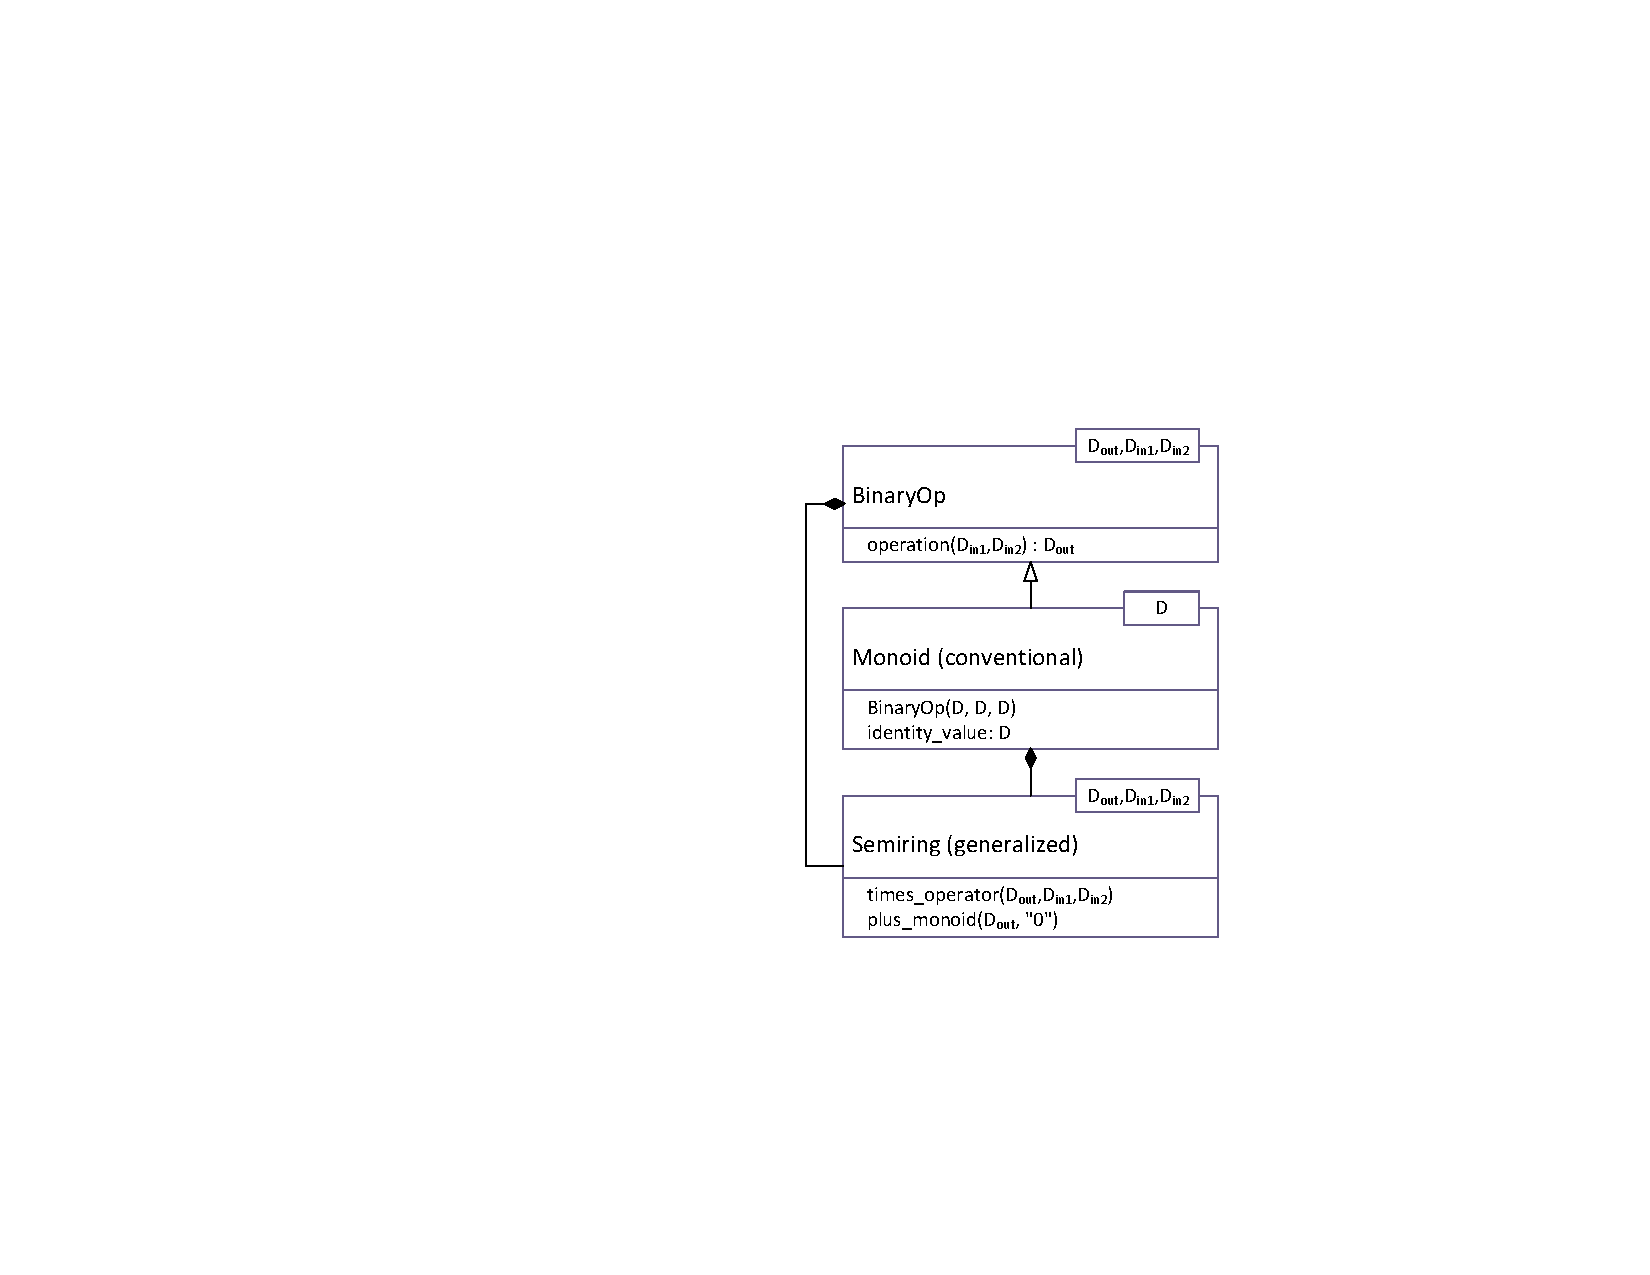
\includegraphics[width=1.0\linewidth,trim=3in 2in 0.5in 2in]{Algebra_Hierarchy_v2_1.pdf}
    \end{center}
    \caption[Hierarchy of algebraic object classes in GraphBLAS.]{Hierarchy of algebraic object classes in GraphBLAS. GraphBLAS 
    semirings consist of a conventional monoid with one domain for the addition 
    function, and a binary operator with three domains for the multiplication function.}
    \label{Fig:AlgebraHierarchy}
    \hrule
\end{figure}

User-defined semirings can be created with calls to {\sf GrB\_Semiring\_new} 
(see Section~\ref{Sec:AlgebraMethods}).
A list of predefined true semirings and convenience
semirings can be found in Tables~\ref{Tab:PredefinedTrueSemirings} and~\ref{Tab:PredefinedUsefulSemirings},
respectively.  Predefined
semirings are named {\sf GrB\_\emph{add}\_\emph{mul}\_SEMIRING\_$T$},
where \emph{add} is the semiring additive operation, \emph{mul} is
the semiring multiplicative operation and $T$ is the domain (type)
of the semiring.

%==================

\begin{table}
\centering
\begin{threeparttable}
\hrule
\caption[Predefined ``true'' semirings for GraphBLAS in C.]{Predefined true semirings 
for GraphBLAS in C where the additive identity is the multiplicative 
annihilator. The $x$ can be one of 8, 16, 32, or 64 in {\sf UINT$x$} or {\sf INT$x$}, 
and can be 32 or 64 in {\sf FP$x$}.}
\label{Tab:PredefinedTrueSemirings}

\hspace*{-1.5em}
\begin{tabular}{l|l|l|l}
                                      & Domains, $T$             & $+$ identity         &                 \\
GraphBLAS identifier              & ($T \times T \rightarrow T$) & $\times$ annihilator & Description     \\ \hline
{\sf GrB\_PLUS\_TIMES\_SEMIRING\_$T$}   & {\sf UINT$x$}            & 0                    & arithmetic semiring \\
                                      & {\sf INT$x$}             & 0                    &                 \\
                                      & {\sf FP$x$}              & 0                    &                 \\
{\sf GrB\_MIN\_PLUS\_SEMIRING\_$T$}     & {\sf UINT$x$}            & {\tt UINT$x$\_MAX}   & min-plus semiring  \\
                                      & {\sf INT$x$}             & {\tt INT$x$\_MAX}    &                 \\
                                      & {\sf FP$x$}              & {\tt INFINITY}       &                 \\
{\sf GrB\_MAX\_PLUS\_SEMIRING\_$T$}     & {\sf INT$x$}             & {\tt INT$x$\_MIN}    & max-plus semiring  \\
                                      & {\sf FP$x$}              & {\tt -INFINITY}      &                 \\
{\sf GrB\_MIN\_TIMES\_SEMIRING\_$T$}    & {\sf UINT$x$}            & {\tt UINT$x$\_MAX}   & min-times semiring \\
{\sf GrB\_MIN\_MAX\_SEMIRING\_$T$}      & {\sf UINT$x$}            & {\tt UINT$x$\_MAX}   & min-max semiring   \\
                                      & {\sf INT$x$}             & {\tt INT$x$\_MAX}    &                 \\
                                      & {\sf FP$x$}              & {\tt INFINITY}       &                 \\
{\sf GrB\_MAX\_MIN\_SEMIRING\_$T$}      & {\sf UINT$x$}            & 0                    & max-min semiring   \\
                                      & {\sf INT$x$}             & {\tt INT$x$\_MIN}    &                 \\
                                      & {\sf FP$x$}              & {\tt -INFINITY}      &                 \\
{\sf GrB\_MAX\_TIMES\_SEMIRING\_$T$}    & {\sf UINT$x$}            & 0                    & max-times semiring \\
{\sf GrB\_PLUS\_MIN\_SEMIRING\_$T$}     & {\sf UINT$x$}            & 0                    & plus-min semiring  \\
                                      &                          &                      &                 \\
{\sf GrB\_LOR\_LAND\_SEMIRING\_BOOL}  & {\sf BOOL}               & {\tt false}          & Logical semiring   \\
{\sf GrB\_LAND\_LOR\_SEMIRING\_BOOL}  & {\sf BOOL}               & {\tt true}           & "and-or" semiring  \\
{\sf GrB\_LXOR\_LAND\_SEMIRING\_BOOL} & {\sf BOOL}               & {\tt false}          & same as {\sf NE\_LAND} \\
{\sf GrB\_LXNOR\_LOR\_SEMIRING\_BOOL} & {\sf BOOL}               & {\tt true}           & same as {\sf EQ\_LOR} \\
\end{tabular}

\hrule
\comment{
\begin{tablenotes}
    \item[1] For {\sf GrB\_ANY\_*\_SEMIRING\_T}, an implementation is free to return any of the results of the application of the "multiply" operator ({\sf FIRST} or {\sf SECOND}), and is not required to always return the same result in different invocations..
\end{tablenotes}
}
\end{threeparttable}
\end{table}

\begin{table}
\centering
\begin{threeparttable}
\hrule
\caption[Other useful predefined semirings for GraphBLAS in C.]{Other useful predefined semirings for GraphBLAS in C that don't have a multiplicative annihilator. 
The $x$ can be one of 8, 16, 32, or 64 in {\sf UINT$x$} or {\sf INT$x$}, 
and can be 32 or 64 in {\sf FP$x$}.}
\label{Tab:PredefinedUsefulSemirings}

\hspace*{-1.5em}
\begin{tabular}{l|l|l|l}
                                    & Domains, $T$             &            &                 \\
GraphBLAS identifier           & ($T \times T \rightarrow T$)  & $+$ identity      & Description             \\ \hline
{\sf GrB\_MAX\_PLUS\_SEMIRING\_$T$}   & {\sf UINT$x$}            & 0                 & max-plus semiring         \\
{\sf GrB\_MIN\_TIMES\_SEMIRING\_$T$}  & {\sf INT$x$}             & {\tt INT$x$\_MAX} & min-times semiring        \\
                                    & {\sf FP$x$}              & {\tt INFINITY}    &                  \\
{\sf GrB\_MAX\_TIMES\_SEMIRING\_$T$}  & {\sf INT$x$}             & {\tt INT$x$\_MIN} & max-times semiring        \\
                                    & {\sf FP$x$}              & {\tt -INFINITY}   &                 \\
{\sf GrB\_PLUS\_MIN\_SEMIRING\_$T$}   & {\sf INT$x$}             & 0                 & plus-min semiring          \\
                                    & {\sf FP$x$}              & 0                 &                 \\ 
{\sf GrB\_MIN\_FIRST\_SEMIRING\_$T$}  & {\sf UINT$x$}            & {\tt UINT$x$\_MAX}& min-select first  semiring     \\
                                    & {\sf INT$x$}             & {\tt INT$x$\_MAX} &                 \\
                                    & {\sf FP$x$}              & {\tt INFINITY}    &                 \\
{\sf GrB\_MIN\_SECOND\_SEMIRING\_$T$} & {\sf UINT$x$}            & {\tt UINT$x$\_MAX}& min-select second semiring     \\
                                    & {\sf INT$x$}             & {\tt INT$x$\_MAX} &                 \\
                                    & {\sf FP$x$}              & {\tt INFINITY}    &                 \\
{\sf GrB\_MAX\_FIRST\_SEMIRING\_$T$}  & {\sf UINT$x$}            & 0                 & max-select first  semiring     \\
                                    & {\sf INT$x$}             & {\tt INT$x$\_MIN} &                 \\
                                    & {\sf FP$x$}              & {\tt -INFINITY}   &                 \\
{\sf GrB\_MAX\_SECOND\_SEMIRING\_$T$} & {\sf UINT$x$}            & 0                 & max-select second semiring     \\
                                    & {\sf INT$x$}             & {\tt INT$x$\_MIN} &                 \\
                                    & {\sf FP$x$}              & {\tt -INFINITY}   &                 \\
\end{tabular}

\hrule
\comment{
\begin{tablenotes}
    \item[1] For {\sf GrB\_ANY\_*\_SEMIRING\_T}, an implementation is free to return any of the results of the application of the "multiply" operator ({\sf FIRST} or {\sf SECOND}), and is not required to always return the same result in different invocations..
\end{tablenotes}
}
\end{threeparttable}
\end{table}

%============================================================================
\section{Collections}

%----------------------------------------------------------------------------
\subsection{Scalars}
\label{Sec:Scalars}

A \emph{GraphBLAS scalar}, $\scalar{s} = \langle D, \{ \sigma \} \rangle$, is defined by
a domain $D$, and a set of zero or one \emph{scalar value}, $\sigma$, where $\sigma \in D$. 
We define $\mathbf{size}(\scalar{s}) = 1$ (constant), and
$\mathbf{L}(\scalar{s}) = \{ \sigma \}$. The set $\mathbf{L}(\scalar{s})$ is
called the \emph{contents} of the GraphBLAS scalar $\scalar{s}$. We also define 
$\mathbf{D}(\scalar{s}) = D$. Finally, $\mathbf{val}(s)$ is a 
reference to the scalar value, $\sigma$, if the GraphBLAS scalar is not empty, and is 
undefined otherwise.

%----------------------------------------------------------------------------
\subsection{Vectors}
\label{Sec:Vectors}

A vector $\vector{v} = \langle D, N, \{ (i,v_i) \} \rangle$ is defined by
a domain $D$, a size $N>0$, and a set of tuples $(i,v_i)$ where $0 \leq
i < N$ and $v_i \in D$. A particular value of $i$ can appear at
most once in $\vector{v}$. We define $\mathbf{size}(\vector{v}) = N$ and
$\mathbf{L}(\vector{v}) = \{ (i,v_i) \}$. The set $\mathbf{L}(\vector{v})$ is
called the \emph{content} of vector $\vector{v}$. We also define the set
$\vector{ind(\vector{v})} = \{ i : (i,v_i) \in \mathbf{L}(\vector{v}) \}$
(called the \emph{structure} of $\vector{v}$), and $\mathbf{D}(\vector{v})
= D$. For a vector $\vector{v}$, $\vector{v}(i)$ is a reference to $v_i$
if $(i,v_i) \in \mathbf{L}(\vector{v})$ and is undefined otherwise.

%----------------------------------------------------------------------------
\subsection{Matrices}
\label{Sec:Matrices}

A matrix $\matrix{A} = \langle D, M, N, \{ (i,j,A_{ij}) \} \rangle$ is
defined by a domain $D$, its number of rows $M>0$, its number of columns
$N>0$, and a set of tuples $(i,j,A_{ij})$ where $0 \leq i < M$, $0 \leq
j < N$, and $A_{ij} \in D$. A particular pair of values $i,j$ can
appear at most once in $\matrix{A}$. We define $\mathbf{ncols}(\matrix{A})
= N$,  $\mathbf{nrows}(\matrix{A}) = M$, and $\mathbf{L}(\matrix{A}) =
\{ (i,j,A_{ij}) \}$.  The set $\mathbf{L}(\matrix{A})$ is called the
\emph{content} of matrix $\matrix{A}$.  We also define the sets
$\vector{indrow(\matrix{A})} = \{ i : \exists (i,j,A_{ij}) \in
\matrix{A} \}$ and $\vector{indcol(\matrix{A})} = \{ j : \exists
(i,j,A_{ij}) \in \matrix{A} \}$.  (These are the sets of nonempty
rows and columns of $\matrix{A}$, respectively.)  The \emph{structure}
of matrix $\matrix{A}$ is the set $\mathbf{ind}(\matrix{A}) = \{ (i,j) :
(i,j,A_{ij}) \in \mathbf{L}(\matrix{A}) \}$, and $\mathbf{D}(\matrix{A}) = D$.
For a matrix $\matrix{A}$, $\matrix{A}(i,j)$ is a reference to $A_{ij}$
if $(i,j,A_{ij}) \in \mathbf{L}(\matrix{A})$ and is undefined otherwise.

If $\matrix{A}$ is a matrix and $0 \leq j < N$, then $\matrix{A}(:,j)
= \langle D, M, \{(i,A_{ij}) : (i,j,A_{ij}) \in \mathbf{L}(\matrix{A})
\} \rangle$ is a vector called the $j$-th \emph{column}
of $\matrix{A}$. Correspondingly, if $\matrix{A}$ is a matrix and
$0 \leq i < M$, then $\matrix{A}(i,:) = \langle D, N, \{(j,A_{ij}) :
(i,j,A_{ij}) \in \mathbf{L}(\matrix{A}) \} \rangle$ is a vector called
the $i$-th \emph{row} of $\matrix{A}$.

Given a matrix $\matrix{A} = \langle D, M, N, \{ (i,j,A_{ij}) \} \rangle$,
its \emph{transpose} is another matrix $\matrix{A}^T = \langle D, N, M, \{
(j,i,A_{ij}) : (i,j,A_{ij}) \in \mathbf{L}(\matrix{A}) \} \rangle$.


%----------------------------------------------------------------------------
\subsection{Masks}
\label{Sec:Masks}

The GraphBLAS C API defines an opaque object called a \emph{mask}.  The mask
is used to control how computed values are stored in the output from a method. 
The mask is an \emph{internal} opaque object; that is, it is never exposed as a 
variable within an application. 

The mask is formed from input objects to the method that uses 
the mask.  For example, a GraphBLAS method may be called with a matrix as the mask
parameter.   The internal mask object is constructed from the input matrix in one
of two ways.  In the default case, an element of the mask is created for each 
tuple that exists in the matrix for which the value of the tuple cast to Boolean 
evaluates to {\tt true}.  Alternatively, the user can specify {\em structure}-only 
behavior where an element of the mask is created for each tuple that exists in 
the matrix {\em regardless} of the value stored in the input matrix.

The internal mask object can be either a one- or a two-dimensional construct.  
One- and two-dimensional masks, described more formally below, are similar to
vectors and matrices, respectively, except that they have structure
(indices) but no values.  When needed, a value is implied for the elements of a 
mask with an implied value of {\tt true} for elements that exist 
and an implied value of {\tt false} for elements that do not exist (\ie,
the locations of the mask that do not have a stored value imply a value of {\tt false}).
Hence, even though a mask does not contain any values, it can be 
considered to imply values from a Boolean domain.

A one-dimensional mask $\vector{m} = \langle N, \{ i \} \rangle$ is
defined by its number of elements $N>0$, and a set $\mathbf{ind}(\vector{m})$
of indices $\{ i \}$ where $0 \leq i < N$.  A particular value of $i$ can
appear at most once in $\vector{m}$. We define $\mathbf{size}(\vector{m})
= N$. The set $\mathbf{ind}(\vector{m})$ is called the \emph{structure} of mask $\vector{m}$.

A two-dimensional mask $\matrix{M} = \langle M, N, \{ (i,j) \}
\rangle$ is defined by its number of rows $M>0$, its number of
columns $N>0$, and a set $\mathbf{ind}(\matrix{M})$ of tuples $(i,j)$
where $0 \leq i < M$, $0 \leq j < N$.   A particular pair of values
$i,j$ can appear at most once in $\matrix{M}$.  We define
$\mathbf{ncols}(\matrix{M}) = N$, and $\mathbf{nrows}(\matrix{M}) = M$.
We also define the sets $\vector{indrow(\matrix{M})} = \{ i : \exists
(i,j) \in \mathbf{ind}(\matrix{M}) \}$ and $\vector{indcol(\matrix{M})}
= \{ j : \exists (i,j) \in \mathbf{ind}(\matrix{M}) \}$.  These are
the sets of nonempty rows and columns of $\matrix{M}$, respectively.
The set $\mathbf{ind}(\matrix{M})$ is called the \emph{structure} of 
mask $\matrix{M}$.

One common operation on masks is the \emph{complement}.
For a one-dimensional mask $\vector{m}$ this is denoted as
$\neg\vector{m}$. For a two-dimensional mask $\matrix{M}$, this is denoted as
$\neg\matrix{M}$.  The complement of a one-dimensional
mask $\vector{m}$ is defined as $\mathbf{ind}(\neg\vector{m}) = \{i : 0
\leq i < N, i \notin \mathbf{ind}(\vector{m}) \}$.  It is the set of all
possible indices that do not appear in $\vector{m}$.  The 
complement of a two-dimensional mask $\matrix{M}$ is defined as the set
$\mathbf{ind}(\neg\matrix{M}) = \{(i,j)$ : $0 \leq i < M$, $0 \leq j < N$,
$(i,j) \notin \mathbf{ind}(\matrix{M}) \}$.  It is the set of all possible
indices that do not appear in $\matrix{M}$.



%-----------------------------------------------------------------------------

%\chapter{Methods \scott{Rename to Operations}}
%\label{Chp:Methods}

%This chapter defines the behavior of all the methods in the GraphBLAS C API.
%All methods can be declared for use in programs by including the {\tt GraphBLAS.h} header file.

%\input{context_methods}

%\section{Object methods}

This section describes methods that setup and operate on GraphBLAS opaque objects
but are not part of the the GraphBLAS math specification.

%\input{algebra_methods}
%\input{scalar_methods}
%\input{vector_matrix_methods}
%\input{descriptor_methods}

\section{GraphBLAS operations}
\label{Sec:Operations}

The GraphBLAS operations are defined in the GraphBLAS math specification and summarized in 
Table~\ref{Tab:GraphBLASOps}.   In addition to methods that implement these
fundamental GraphBLAS operations, we support a number of variants that have been 
found to be especially useful in algorithm development.
A flowchart of the overall behavior of a GraphBLAS operation is shown 
in Figure~\ref{Fig:mxmFlowchart}.

\begin{table}[p]
\hrule
\begin{center}
\caption[A mathematical notation for the fundamental GraphBLAS operations 
supported in this specification.]{A mathematical notation for the fundamental GraphBLAS operations 
supported in this specification.  Input matrices $\matrix{A}$ and $\matrix{B}$ 
may be optionally transposed (not shown). Use of an optional accumulate with 
existing values in the output object is indicated with $\odot$.  Use of optional write 
masks and replace flags are indicated as $\matrix{C}\langle\matrix{M},r\rangle$ 
when applied to the output matrix, $\matrix{C}$.  The mask controls which values 
resulting from the operation on the right-hand side are written into the output 
object (complement and structure flags are not shown).  The ``replace'' 
option, indicated by specifying the $r$ flag, means that all values in the 
output object are removed prior to assignment. If ``replace'' is not specified, 
only the values/locations computed on the right-hand side and allowed by the 
mask will be written to the output (``merge'' mode).}
\label{Tab:GraphBLASOps}
~\\
\newcommand{\odotsp}{\hspace{-0.2cm}\odot\hspace{-0.18cm}}
\begin{tabular}{l|rcrcl}
{\sf Operation Name} & \multicolumn{5}{c}{Mathematical Notation}  \\
\hline
{\sf mxm}          & $\matrix{C}\langle\matrix{M},r\rangle$ & $=$ & $\matrix{C}$ & $\odotsp$ & $\matrix{A} \oplus.\otimes \matrix{B}$  \\
{\sf mxv}          & $\vector{w}\langle\vector{m},r\rangle$ & $=$ & $\vector{w}$ & $\odotsp$ & $\matrix{A} \oplus.\otimes \vector{u}$  \\
{\sf vxm}          & $\vector{w}^T\langle\vector{m}^T,r\rangle$ & $=$ & \hspace{-0.18cm}$\vector{w}^T$ & $\odotsp$ & $\vector{u}^T \oplus.\otimes \matrix{A}$  \\
{\sf eWiseMult}    & $\matrix{C}\langle\matrix{M},r\rangle$ & $=$ & $\matrix{C}$ & $\odotsp$ & $\matrix{A} \otimes \matrix{B}$  \\
                   & $\vector{w}\langle\matrix{m},r\rangle$ & $=$ & $\vector{w}$ & $\odotsp$ & $\vector{u} \otimes \vector{v}$  \\
{\sf eWiseAdd}     & $\matrix{C}\langle\matrix{M},r\rangle$ & $=$ & $\matrix{C}$ & $\odotsp$ & $\matrix{A} \oplus  \matrix{B}$  \\
                   & $\vector{w}\langle\matrix{m},r\rangle$ & $=$ & $\vector{w}$ & $\odotsp$ & $\vector{u} \oplus \vector{v}$  \\
{\sf extract}      & $\matrix{C}\langle\matrix{M},r\rangle$ & $=$ & $\matrix{C}$ & $\odotsp$ & $\matrix{A}(\grbarray{i},\grbarray{j})$ \\
                   & $\vector{w}\langle\matrix{m},r\rangle$ & $=$ & $\vector{w}$ & $\odotsp$ & $\vector{u}(\grbarray{i})$ \\
%{\sf extract} (column) & $\matrix{w}\langle\vector{m},r\rangle$ & $=$ & $\matrix{w}$ & $\odotsp$ & $\matrix{A}(\grbarray{i}, j)$ \\
{\sf assign}       & $\matrix{C}\langle\matrix{M},r\rangle(\grbarray{i},\grbarray{j})$ & $=$ & $\matrix{C}(\grbarray{i},\grbarray{j})$ & $\odotsp$ & $\matrix{A}$ \\
                   & $\vector{w}\langle\vector{m},r\rangle(\grbarray{i})$ & $=$ & $\vector{w}(\grbarray{i})$ & $\odotsp$ & $\matrix{u}$ \\
{\sf reduce} (row) & $\vector{w}\langle\vector{m},r\rangle$ & $=$ & $\vector{w}$ & $\odotsp$ & $\left[\oplus_j\matrix{A}(:,j)\right]$  \\
{\sf reduce} (scalar) & $s$ & $=$ & $s$ & $\odotsp$ & $\left[\oplus_{i,j}\matrix{A}(i,j) \right]$  \\
                      & $s$ & $=$ & $s$ & $\odotsp$ & $\left[\oplus_i\matrix{u}(i) \right]$  \\
{\sf apply}        & $\matrix{C}\langle\matrix{M},r\rangle$ & $=$ & $\matrix{C}$ & $\odotsp$ & $f_u(\matrix{A})$ \\
                   & $\vector{w}\langle\matrix{m},r\rangle$ & $=$ & $\vector{w}$ & $\odotsp$ & $f_u(\vector{u} )$  \\
\hline
{\sf apply(indexop)}     & $\matrix{C}\langle\matrix{M},r\rangle$ & $=$ & $\matrix{C}$ & $\odotsp$ & $f_{i}(\matrix{A},\mathbf{ind}(\matrix{A}),s)$ \\
                   & $\vector{w}\langle\matrix{m},r\rangle$ & $=$ & $\vector{w}$ & $\odotsp$ & $f_{i}(\vector{u},\mathbf{ind}(\vector{u}),s)$  \\
{\sf select  }     & $\matrix{C}\langle\matrix{M},r\rangle$ & $=$ & $\matrix{C}$ & $\odotsp$ & $\matrix{A}\langle f_{i}(\matrix{A},\mathbf{ind}(\matrix{A}),s)\rangle$ \\
                   & $\vector{w}\langle\matrix{m},r\rangle$ & $=$ & $\vector{w}$ & $\odotsp$ & $\vector{u}\langle f_{i}(\vector{u},\mathbf{ind}(\vector{u}),s)\rangle$  \\
\hline
{\sf transpose}    & $\matrix{C}\langle\matrix{M},r\rangle$ & $=$ & $\matrix{C}$ & $\odotsp$ & $\matrix{A}^T$ \\
{\sf kronecker}          & $\matrix{C}\langle\matrix{M},r\rangle$ & $=$ & $\matrix{C}$ & $\odotsp$ & $\matrix{A}  \kron \matrix{B}$  \\
%& & & \\
%& \multicolumn{3}{c}{Input/Output Operations} \\
%{\sf Matrix\_build}  & $\matrix{C}$ & $=$ & $\mathbb{S}^{m\times n}(\grbarray{i},\grbarray{j},\grbarray{v},\oplus_{dup})$ \\
%{\sf Vector\_build}  & $\vector{w}$ & $=$ & $\mathbb{S}^{n}(\grbarray{i},\grbarray{v},\oplus_{dup})$ \\
%{\sf Matrix\_extractTuples} & $(\grbarray{i},\grbarray{j},\grbarray{v})$ & $=$ & $\matrix{A}$ \\
%{\sf Vector\_extractTuples} & $(\grbarray{i},\grbarray{v})$ & $=$ & $\matrix{u}$ \\
\end{tabular}
\end{center}
\hrule
\end{table}

\begin{figure}[p]
    \hrule
    \begin{center}
        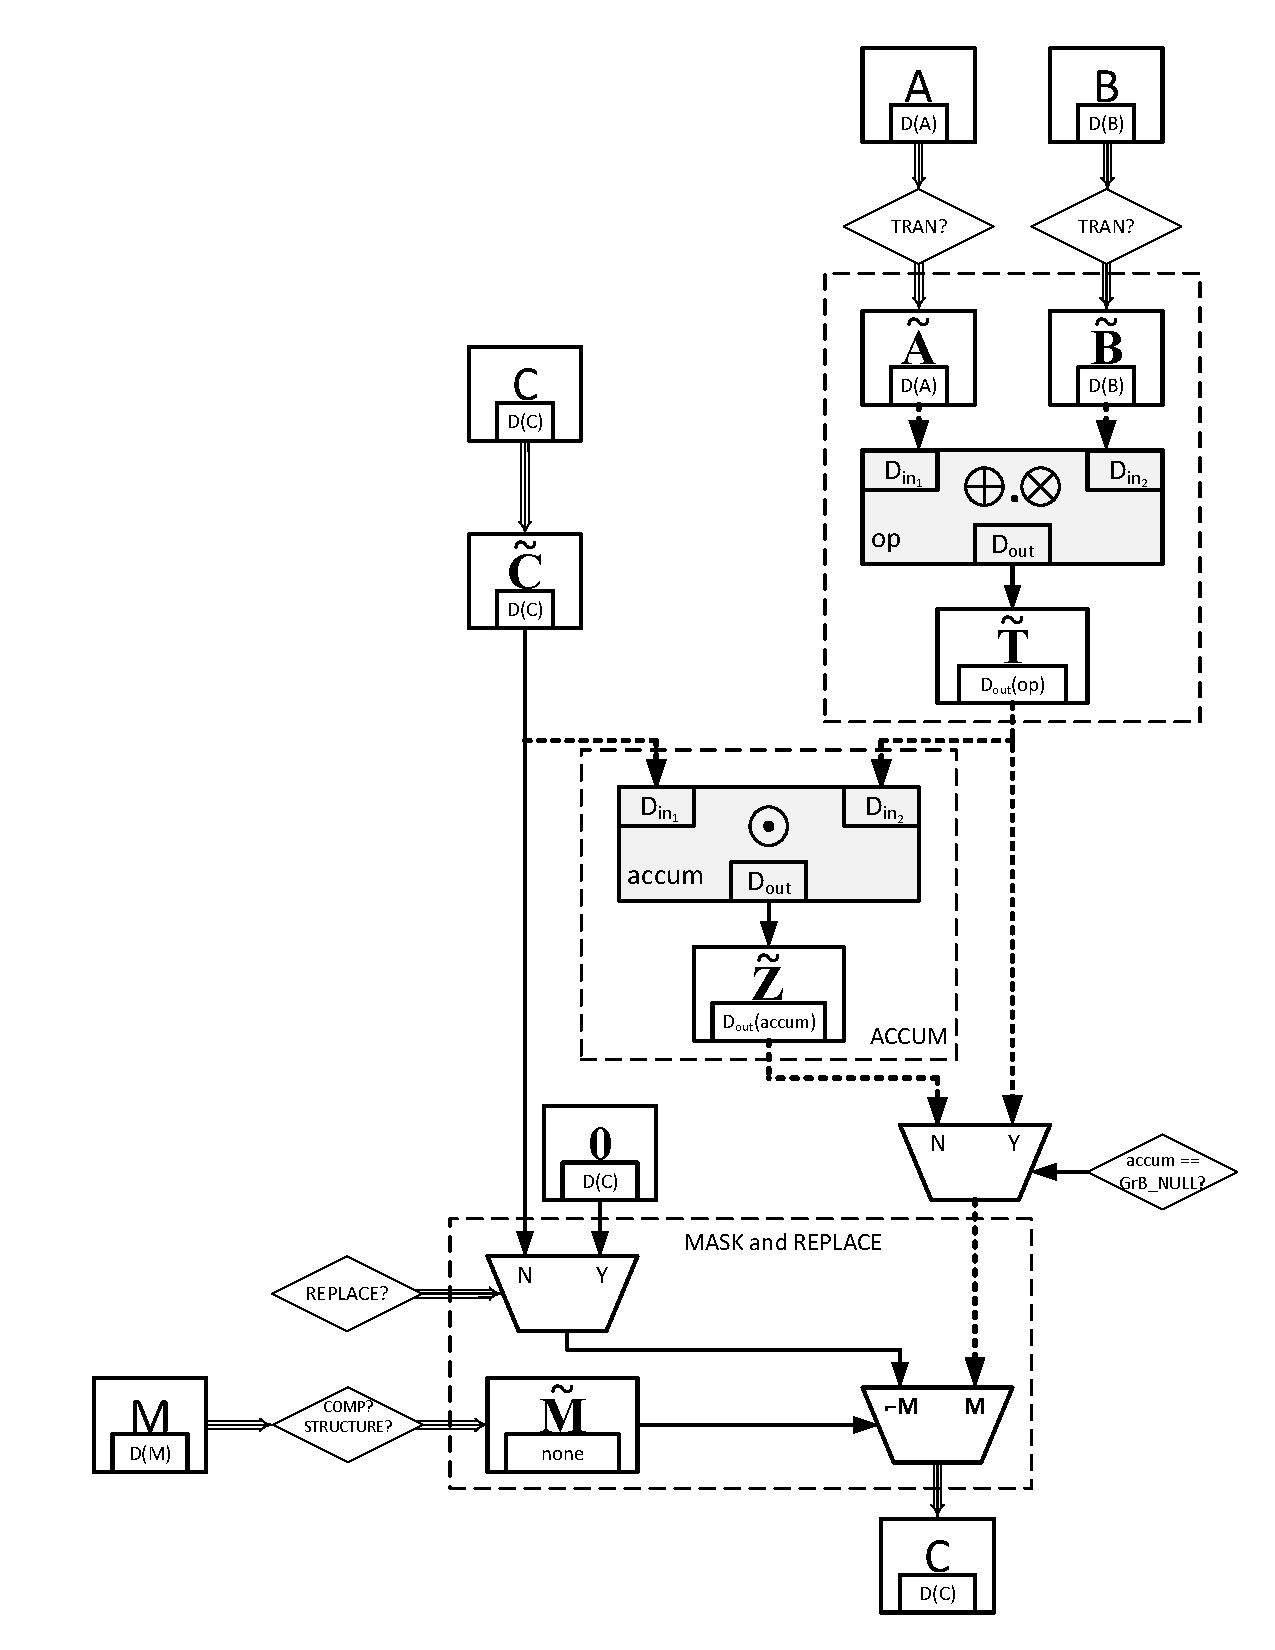
\includegraphics[width=5.5in]{mxm_operation_flowchart_1_3d.pdf}
    \end{center}
    \caption[Flowchart for the GraphBLAS operations.]{Flowchart for the GraphBLAS operations. Although shown specifically for
	the {\sf mxm} operation, many elements are common to all operations: such as the 
	``{\sf ACCUM}'' and ``{\sf MASK and REPLACE}'' blocks.  The triple arrows 
    ($\Rrightarrow$) denote where ``as if copy'' takes place (including both 
    collections and descriptor settings).  The bold, dotted arrows indicate
    where casting may occur between different domains.}
    \label{Fig:mxmFlowchart}
    \hrule
\end{figure}

\paragraph{Domains and Casting}

A GraphBLAS operation is only valid when the domains of the GraphBLAS objects are
mathematically consistent.  The C programming language defines implicit casts 
between built-in data types.  For example, {\sf float}s, {\sf double}s, and {\sf int}s can be 
freely mixed according to the rules defined for implicit casts.  It is the 
responsibility of the user to assure that these casts are appropriate for the 
algorithm in question.  For example, a cast to {\sf int} implies truncation of a floating 
point type.  Depending on the operation, this truncation error could lead to
erroneous results.  Furthermore, casting a wider type onto a narrower type can lead 
to overflow errors.  The GraphBLAS operations do not attempt to protect a user from 
these sorts of errors.

When user-define types are involved, however, GraphBLAS requires strict equivalence
between types and no casting is supported.  If GraphBLAS detects these mismatches,
it will return a domain mismatch error.

\paragraph{Dimensions and Transposes}

GraphBLAS operations also make assumptions about the numbers of dimensions and 
the sizes of vectors and matrices in an operation.   An operation will test these 
sizes and report an error if they are not \emph{shape compatible}.  For example, when multiplying 
two matrices, $\matrix{C} = \matrix{A} \times \matrix{B}$, the number of rows of 
$\matrix{C}$ must equal the number of rows of $\matrix{A}$, the number of columns 
of $\matrix{A}$ must match the number of rows of $\matrix{B}$, and the number of 
columns of $\matrix{C}$ must match the number of columns of $\matrix{B}$.  This 
is the behavior expected given the mathematical definition of the operations.   

For most of the GraphBLAS operations involving matrices, an optional descriptor 
can modify the matrix associated with an input GraphBLAS matrix object.  For 
example, if an input matrix is an argument to a GraphBLAS operation and the 
associated descriptor indicates the transpose option, then the operation occurs 
as if on the transposed matrix.  In this case, the relationships between the 
sizes in each dimension shift in the mathematically expected way. 


\paragraph{Compliance}

We follow a \emph{prescriptive} approach to the definition of the semantics
of GraphBLAS operations. That is, for each operation we give a recipe for
producing its outcome.
Any implementation that produces the same outcome,
and follows the GraphBLAS execution model (Section~\ref{Sec:ExecutionModel}) and
error model (Section~\ref{Sec:ErrorModel}) is a conforming implementation.


%-----------------------------------------------------------------------------
\section{Matrix multiplication (and vector multiplication?}

Should we add vxv which is dot product?

%-----------------------------------------------------------------------------
\subsection{{\sf mxm}: Matrix-matrix multiply}

Multiplies a matrix with another matrix on a semiring. The result is a matrix.

\paragraph{\syntax}

$$
\matrix{T} ~ = ~ \matrix{A}^{[T]} \oplus.\otimes \matrix{B}^{[T]}
$$

\paragraph{Where:}

\begin{itemize}[leftmargin=0.7in]
    \item[$\matrix{A}^{[T]}$]    ({\sf IN}) $\in \mathbb{D}_A^{n\times k}$

    \item[$\matrix{B}^{[T]}$]    ({\sf IN}) $\in \mathbb{D}_B^{k\times m}$

    \item[$\oplus.\otimes$]   ({\sf IN}) The semiring used in the matrix
    multiplication, $\langle \mathbb{D}_\oplus, \mathbb{D}_{in1},\mathbb{D}_{in2},\oplus,\otimes,0 \rangle$.

    \item[$\matrix{T}$]    ({\sf OUT}) $\in \mathbb{D}_\oplus^{n\times m}$
    
\end{itemize}


\paragraph{Description}

{\sf mxm} computes the matrix product 
$\matrix{T} = \matrix{A}^{[T]} \oplus . \otimes \matrix{B}^{[T]}$
(where matrices \matrix{A} and \matrix{B} can be optionally transposed).  

\scott{Definitions/notation of each matrix omitted, define once earlier if at all.}

\scott{Domain compatibility b/w containers and operators omitted, define once earlier.}


From the argument matrices, the internal matrices used in 
the computation are formed ($\leftarrow$ denotes copy): \scott{Find a notation that does not refer to descriptors (descriptors is an implementation detail not math).}
\begin{enumerate}

	\item Matrix $\matrix{\widetilde{A}} \leftarrow
    {\sf desc[GrB\_INP0].GrB\_TRAN} \ ? \ \matrix{A}^T : \matrix{A}$.

	\item Matrix $\matrix{\widetilde{B}} \leftarrow
    {\sf desc[GrB\_INP1].GrB\_TRAN} \ ? \ \matrix{B}^T : \matrix{B}$.
\end{enumerate}

\scott{Dimension compatibility checks omitted.}

We are now ready to carry out the matrix multiplication.
The intermediate matrix \\
$\matrix{\widetilde{T}} = \langle
\bDout({\sf op}), \bold{nrows}(\matrix{\widetilde{A}}), \bold{ncols}(\matrix{\widetilde{B}}),
\{(i,j,T_{ij}) : \bold{ind}(\matrix{\widetilde{A}}(i,:)) \cap
\bold{ind}(\matrix{\widetilde{B}}(:,j)) \neq \emptyset \} \rangle$
is created.  The value of each of its elements is computed by 
\[T_{ij} = \bigoplus_{k \in \bold{ind}(\matrix{\widetilde{A}}(i,:)) \cap
\bold{ind}(\matrix{\widetilde{B}}(:,j))} (\matrix{\widetilde{A}}(i,k)
\otimes \matrix{\widetilde{B}}(k,j)),\] where $\oplus$ and $\otimes$
are the additive and multiplicative operators of semiring {\sf op},
respectively.

\scott{Is the following describe possibilities in the realm of math?}
\begin{itemize}
\item if $\oplus$ is commutative and associative no order is imposed on the elements of the intersection set.
\item if $\oplus$ is not commutative then the order must be from lowest to highest index $k$. Arbitrary grouping is allowed as long as relative order is maintained.
\item if $\oplus$ is neither commutative nor associative, strictly sequential and ordered operation is required.
\end{itemize}

%-----------------------------------------------------------------------------

\subsection{{\sf vxm}: Vector-matrix multiply}

Multiplies a (row) vector with a matrix on an semiring. The result is a vector.

\paragraph{\syntax}

$$
\vector{t}^T ~ = ~ \vector{u}^{T} \oplus.\otimes \matrix{A}^{[T]}
$$

\paragraph{Where:}

\begin{itemize}[leftmargin=1.1in]
    \item[$\vector{u}$]    ({\sf IN}) $\in \mathbb{D}_{u}^{n}$

    \item[$\matrix{A}^{[T]}$]    ({\sf IN}) $\in \mathbb{D}_A^{n\times m}$

    \item[$\oplus.\otimes$]   ({\sf IN}) The semiring used in the matrix
    multiplication, $\langle \mathbb{D}_\oplus, \mathbb{D}_{in1},\mathbb{D}_{in2},\oplus,\otimes,0 \rangle$.

    \item[$\vector{t}$]    ({\sf OUT}) $\in \mathbb{D}_\oplus^{m}$

\end{itemize}

\paragraph{Description}

{\sf vxm} computes the vector-matrix product 
$\vector{t}^T = \vector{u}^T \oplus . \otimes \matrix{A}^{[T]}$ 
(where matrix \matrix{A} can be optionally transposed).

\scott{Definitions/notation of each matrix and vector omitted, define once earlier if at all.}

\scott{Domain compatibility b/w containers and operators omitted, define once earlier.}


From the argument vectors and matrices, the internal matrices and vectors used in 
the computation are formed ($\leftarrow$ denotes copy): \scott{Find a notation that does not refer to descriptors (descriptors is an implementation detail not math).}
\begin{enumerate}
	\item Vector $\vector{\widetilde{u}} \leftarrow \vector{u}$.

	\item Matrix $\matrix{\widetilde{A}} \leftarrow {\sf desc[GrB\_INP1].GrB\_TRAN} \ ? \ \matrix{A}^T : \matrix{A}$.
\end{enumerate}

\scott{Dimension compatibility checks omitted.}


We are now ready to carry out the vector-matrix multiplication.

The intermediate vector $\vector{\widetilde{t}} = \langle
\bDout({\sf op}), \bold{ncols}(\matrix{\widetilde{A}}),
\{(j,t_j) : \bold{ind}(\vector{\widetilde{u}}) \cap
\bold{ind}(\matrix{\widetilde{A}}(:,j)) \neq \emptyset \} \rangle$
is created.  The value of each of its elements is computed by 
\[t_j = \bigoplus_{k \in \bold{ind}(\vector{\widetilde{u}}) \cap
\bold{ind}(\matrix{\widetilde{A}}(:,j))} (\vector{\widetilde{u}}(k)
\otimes \matrix{\widetilde{A}}(k,j)),\] where $\oplus$ and $\otimes$
are the additive and multiplicative operators of semiring {\sf op},
respectively.

\scott{Same comments about associativity and commutativity.}

%-----------------------------------------------------------------------------

\subsection{{\sf mxv}: Matrix-vector multiply}

Multiplies a matrix by a vector on a semiring. The result is a vector.

\paragraph{\syntax}

$$
\vector{t}~ = ~ \matrix{A}^{[T]} \oplus.\otimes \vector{u}
$$

where

\begin{itemize}[leftmargin=1.1in]
    \item[$\matrix{A}^{[T]}$]    ({\sf IN}) $\in \mathbb{D}_A^{n\times m}$

    \item[$\vector{u}$]    ({\sf IN}) $\in \mathbb{D}_{u}^{m}$

    \item[$\oplus.\otimes$]   ({\sf IN}) The semiring used in the matrix
    multiplication, $\langle \mathbb{D}_\oplus, \mathbb{D}_{in1},\mathbb{D}_{in2},\oplus,\otimes,0 \rangle$.

    \item[$\vector{t}$]    ({\sf OUT}) $\in \mathbb{D}_\oplus^{n}$
\end{itemize}

\paragraph{Description}

{\sf mxv} computes the matrix-vector product $\vector{t} = \matrix{A}
\oplus . \otimes \vector{u}$ (where matrix \matrix{A}
 can be optionally transposed).

\scott{Definitions/notation of each matrix and vector omitted, define once earlier if at all.}

\scott{Domain compatibility b/w containers and operators omitted, define once earlier.}

From the argument vectors and matrices, the internal matrices and mask used in 
the computation are formed ($\leftarrow$ denotes copy):  \scott{Find a notation that does not refer to descriptors (descriptors is an implementation detail not math).}
\begin{enumerate}
	\item Matrix $\matrix{\widetilde{A}} \leftarrow {\sf desc[GrB\_INP0].GrB\_TRAN} \ ? \ \matrix{A}^T : \matrix{A}$.

	\item Vector $\vector{\widetilde{u}} \leftarrow \vector{u}$.
\end{enumerate}

\scott{Dimension compatibility checks omitted.}

We are now ready to carry out the matrix-vector multiplication.

The intermediate vector $\vector{\widetilde{t}} = \langle
\bDout({\sf op}), \bold{nrows}(\matrix{\widetilde{A}}),
\{(i,t_i) : \bold{ind}(\matrix{\widetilde{A}}(i,:)) \cap 
\bold{ind}(\vector{\widetilde{u}}) \neq \emptyset \} \rangle$
is created.  The value of each of its elements is computed by 
\[t_i = \bigoplus_{k \in \bold{ind}(\matrix{\widetilde{A}}(i,:)) \cap
\bold{ind}(\vector{\widetilde{u}})} (\matrix{\widetilde{A}}(i,k)
\otimes \vector{\widetilde{u}}(k)),\] where $\oplus$ and $\otimes$
are the additive and multiplicative operators of semiring {\sf op},
respectively.

\scott{Same comments about associativity and commutativity.}

%-----------------------------------------------------------------------------

\subsection{Proposal: {\sf vxv}: vector dot product}

Multiplies a vector by a vector on a semiring. The result is a scalar.

\paragraph{\syntax}

$$
t ~ = ~ \vector{u}^T \oplus.\otimes \vector{v}
$$

%%-----------------------------------------------------------------------------
\section{Element-wise multiplication or intersection}

{\sf eWiseMult} returns an object whose indices are the ``intersection'' of 
the indices of the inputs. The operator is invoked when scalars from two 
operands are present.

%-----------------------------------------------------------------------------

\subsection{{\sf eWiseMult/Intersect}: Vector variant}

Perform element-wise (general) multiplication on the intersection of elements 
of two vectors, producing a third vector as result.

\paragraph{\syntax}

$$
\matrix{T} ~ = ~ \vector{u} \otimes \vector{v}
$$

where

\begin{itemize}[leftmargin=1.1in]
    \item[$\vector{u}$]    ({\sf IN}) $\in \mathbb{D}_{u}^{n}$

    \item[$\vector{v}$]    ({\sf IN}) $\in \mathbb{D}_{v}^{n}$

    \item[$\otimes$]   ({\sf IN}) binary operator to combine values, $\mathbb{D}_{in1} \times \mathbb{D}_{in2} \rightarrow \mathbb{D}_\otimes$.  It does not need to commutative or associative.

    \item[$\matrix{T}$]    ({\sf OUT}) $\in \mathbb{D}_\otimes^{n}$

\end{itemize}

\paragraph{Description}

This variant of {\sf eWiseMult} or {\sf Intersect} computes the element-wise ``product'' or 
``intersection'' of two vectors given a specified binary operator, 
$\otimes$: $\matrix{T} = \vector{u} \otimes \vector{v}$.  Assuming the domains of the
elements in the vectors and the domains expected by the operator are compatible
and the sizes of the vectors are the same.

From the argument vectors, the internal vectors used in 
the computation are formed ($\leftarrow$ denotes copy):
\begin{enumerate}
	\item Vector $\vector{\widetilde{u}} \leftarrow \vector{u}$.

	\item Vector $\vector{\widetilde{v}} \leftarrow \vector{v}$.
\end{enumerate}

We are now ready to carry out the element-wise ``product''.

The intermediate vector $\vector{\widetilde{t}} = \langle
\bDout({\sf op}), \bold{size}(\vector{\widetilde{u}}),
\{(i,t_i) : \bold{ind}(\vector{\widetilde{u}}) \cap 
\bold{ind}(\vector{\widetilde{v}})
 \neq \emptyset \} \rangle$
is created.  The value of each of its elements is computed by:
\[t_i = (\vector{\widetilde{u}}(i)
\otimes \vector{\widetilde{v}}(i)), \forall i \in 
(\bold{ind}(\vector{\widetilde{u}}) \cap 
\bold{ind}(\vector{\widetilde{v}}))\]

%-----------------------------------------------------------------------------

\subsection{{\sf eWiseMult/Intersect}: Matrix variant}

Perform element-wise (general) multiplication on the intersection of elements 
of two matrices, producing a third matrix as result.

\paragraph{\syntax}


$$
\matrix{T} ~ = ~ \matrix{A}^{[T]} \otimes \matrix{B}^{[T]}
$$

where

\begin{itemize}[leftmargin=1.1in]
    \item[$\matrix{A}^{[T]}$]    ({\sf IN}) $\in \mathbb{D}_{A}^{n\times m}$

    \item[$\matrix{B}^{[T]}$]    ({\sf IN}) $\in \mathbb{D}_{B}^{n\times m}$

    \item[$\otimes$]   ({\sf IN}) binary operator to combine values, $\mathbb{D}_{in1} \times \mathbb{D}_{in2} \rightarrow \mathbb{D}_\otimes$.  It does not need to commutative nor associative.

    \item[$\matrix{T}$]    ({\sf OUT}) $\in \mathbb{D}_\otimes^{n\times m}$
\end{itemize}


\paragraph{Description}

This variant of {\sf eWiseMult} or {\sf Intersect} computes the element-wise ``product'' of
two matrices: $\matrix{T} = \matrix{A} \otimes \matrix{B}$.  Assuming the domains of the
elements in the matrices and the domains expected by the operator are compatible
and the sizes of the matrices (after optional transposes) are the same.

From the argument matrices, the internal matrices used in 
the computation are formed ($\leftarrow$ denotes copy): \scott{Find a notation that does not refer to descriptors (descriptors is an implementation detail not math).}
\begin{enumerate}
	\item Matrix $\matrix{\widetilde{A}} \leftarrow
    {\sf desc[GrB\_INP0].GrB\_TRAN} \ ? \ \matrix{A}^T : \matrix{A}$.

	\item Matrix $\matrix{\widetilde{B}} \leftarrow
    {\sf desc[GrB\_INP1].GrB\_TRAN} \ ? \ \matrix{B}^T : \matrix{B}$.
\end{enumerate}

The intermediate matrix $\matrix{\widetilde{T}} = \langle
\bDout({\sf op}), \bold{nrows}(\matrix{\widetilde{A}}), \bold{ncols}(\matrix{\widetilde{A}}),
\{(i,j,T_{ij}) : \bold{ind}(\matrix{\widetilde{A}}) \cap 
\bold{ind}(\matrix{\widetilde{B}}) \neq \emptyset \} \rangle$
is created.  The value of each of its elements is computed by 
\[T_{ij} = (\matrix{\widetilde{A}}(i,j)
\otimes \matrix{\widetilde{B}}(i,j)), \forall (i,j) \in 
\bold{ind}(\matrix{\widetilde{A}}) \cap 
\bold{ind}(\matrix{\widetilde{B}})\]

%=============================================================================
%-----------------------------------------------------------------------------
\section{Element-wise addition or union}

{\sf eWiseAdd} returns an object whose set of indices are the ``union'' of the 
indices of the input operand. The operator is invoked when scalars from two 
operands are present (either stored in the matrix or in the optional variant: 
passed as the fill-in value).


%-----------------------------------------------------------------------------
\subsection{{\sf eWiseAdd/Union}: Vector variant}

Perform element-wise (general) addition on the elements of two vectors,
producing a third vector as result.

\paragraph{\syntax}

\begin{eqnarray*}
\matrix{T} & = & \vector{u} \oplus \vector{v} \\
\matrix{T} & = & \left\{ \vector{u}\cup u_0 \right\} \oplus \left\{ \vector{v} \cup v_0 \right\}  \mbox{~~~(providing missing values)}
\end{eqnarray*}

where

\begin{itemize}[leftmargin=1.1in]
    \item[$\vector{u}$]    ({\sf IN}) $\in \mathbb{D}_{u}^{n}$

    \item[$\vector{v}$]    ({\sf IN}) $\in \mathbb{D}_{v}^{n}$

    \item[$\oplus$]   ({\sf IN}) binary operator to combine values, $\mathbb{D}_{in1} \times \mathbb{D}_{in2} \rightarrow \mathbb{D}_\oplus$.  It does not need to commutative or associative.

    \item[$\matrix{T}$]    ({\sf OUT}) $\in \mathbb{D}_\oplus^{n}$

\end{itemize}

\paragraph{Description}

This variant of {\sf eWiseAdd} or {\sf Union} computes the element-wise ``sum'' or
``union'' of two vectors given the specified binary operator, $\oplus$: 
$\matrix{T} = \vector{u} \oplus \vector{v}$.  Assuming the domains of the
elements in the vectors and the domains expected by the operator are compatible
and the sizes of the vectors are the same.

From the argument vectors, the internal vectors used in 
the computation are formed ($\leftarrow$ denotes copy):
\begin{enumerate}
	\item Vector $\vector{\widetilde{u}} \leftarrow \vector{u}$.

	\item Vector $\vector{\widetilde{v}} \leftarrow \vector{v}$.
\end{enumerate}

We are now ready to carry out the element-wise ``sum''.

The intermediate vector $\vector{\widetilde{t}} = \langle
\bDout({\sf op}), \bold{size}(\vector{\widetilde{u}}),
\{(i,t_i) : \bold{ind}(\vector{\widetilde{u}}) \cup 
\bold{ind}(\vector{\widetilde{v}})
 \neq \emptyset \} \rangle$
is created.  The value of each of its elements is computed by:
\begin{eqnarray*}
t_i & = & 
\begin{cases}
 \vector{\widetilde{u}}(i) \oplus \vector{\widetilde{v}}(i), & \forall i \in (\bold{ind}(\vector{\widetilde{u}}) \cap \bold{ind}(\vector{\widetilde{v}}))\\
 \vector{\widetilde{u}}(i), & \forall i \in (\bold{ind}(\vector{\widetilde{u}}) - (\bold{ind}(\vector{\widetilde{u}}) \cap \bold{ind}(\vector{\widetilde{v}})))\\
  \vector{\widetilde{v}}(i), & \forall i \in (\bold{ind}(\vector{\widetilde{v}}) - (\bold{ind}(\vector{\widetilde{u}}) \cap \bold{ind}(\vector{\widetilde{v}})))
\end{cases}
\end{eqnarray*}
where the difference operator in the previous expressions refers to set difference.

In the case where $u_0$ and $v_0$ scalars are specified they are used when only
one of the vector operands has a stored value at a particular location (and the other does).  
The value of each of its elements is computed by:
\begin{eqnarray*}
t_i & = & 
\begin{cases}
 \vector{\widetilde{u}}(i) \oplus \vector{\widetilde{v}}(i), & \forall i \in (\bold{ind}(\vector{\widetilde{u}}) \cap \bold{ind}(\vector{\widetilde{v}}))\\
 \vector{\widetilde{u}}(i) {\color{red}~ \oplus ~ v_0}, & \forall i \in (\bold{ind}(\vector{\widetilde{u}}) - (\bold{ind}(\vector{\widetilde{u}}) \cap \bold{ind}(\vector{\widetilde{v}})))\\

 {\color{red} u_0 ~\oplus ~}\vector{\widetilde{v}}(i), & \forall i \in (\bold{ind}(\vector{\widetilde{v}}) - (\bold{ind}(\vector{\widetilde{u}}) \cap \bold{ind}(\vector{\widetilde{v}})))
\end{cases}
\end{eqnarray*}
where the difference operator in the previous expressions refers to set difference.


%-----------------------------------------------------------------------------

\subsection{{\sf eWiseAdd/Union}: Matrix variant}

Perform element-wise (general) addition on the elements of two matrices,
producing a third matrix as result.

\paragraph{\syntax}

\begin{eqnarray*}
\matrix{T} & = & \matrix{A}^{[T]} \oplus \matrix{B}^{[T]} \\
\matrix{T} & = & \left\{ \matrix{A}^{[T]}\cup a_0 \right\} \oplus \left\{ \matrix{B}^{[T]} \cup b_0 \right\}  \mbox{~~~(providing missing values)}
\end{eqnarray*}

where

\begin{itemize}[leftmargin=1.1in]
    \item[$\matrix{A}^{[T]}$]    ({\sf IN}) $\in \mathbb{D}_{A}^{n\times m}$

    \item[$\matrix{B}^{[T]}$]    ({\sf IN}) $\in \mathbb{D}_{B}^{n\times m}$

    \item[$\oplus$]   ({\sf IN}) binary operator to combine values, $\mathbb{D}_{in1} \times \mathbb{D}_{in2} \rightarrow \mathbb{D}_\oplus$.  It does not need to commutative or associative.

    \item[$\matrix{T}$]    ({\sf OUT}) $\in \mathbb{D}_\otimes^{n\times m}$
\end{itemize}

\paragraph{Description}

This variant of {\sf eWiseAdd} or {\sf Union} computes the element-wise ``sum'' or
``union'' of two matrices given the specified binary operator, $\oplus$: 
$\matrix{T} = {\sf A} \oplus {\sf B}$.  Assuming the domains of the
elements in the matrices and the domains expected by the operator are compatible
and the sizes of the matrices are the same.

From the argument matrices, the internal matrices used in 
the computation are formed ($\leftarrow$ denotes copy): \scott{Find a notation that does not refer to descriptors (descriptors is an implementation detail not math).}
\begin{enumerate}	\item Matrix $\matrix{\widetilde{A}} \leftarrow
    {\sf desc[GrB\_INP0].GrB\_TRAN} \ ? \ {\sf A}^T : {\sf A}$.

	\item Matrix $\matrix{\widetilde{B}} \leftarrow
    {\sf desc[GrB\_INP1].GrB\_TRAN} \ ? \ {\sf B}^T : {\sf B}$.
\end{enumerate}

The intermediate matrix $\matrix{\widetilde{T}} = \langle
\bDout({\sf op}), \bold{nrows}(\matrix{\widetilde{A}}), \bold{ncols}(\matrix{\widetilde{A}}),
\{(i,j,T_{ij}) : \bold{ind}(\matrix{\widetilde{A}}) \cup 
\bold{ind}(\matrix{\widetilde{B}}) \neq \emptyset \} \rangle$
is created.  The value of each of its elements is computed by :
\begin{eqnarray*}
T_{ij} & = & 
\begin{cases}
 (\matrix{\widetilde{A}}(i,j) \oplus \matrix{\widetilde{B}}(i,j)),& \forall (i,j) \in \bold{ind}(\matrix{\widetilde{A}}) \cap \bold{ind}(\matrix{\widetilde{B}})\\
 \matrix{\widetilde{A}}(i,j),& \forall (i,j) \in (\bold{ind}(\matrix{\widetilde{A}}) - (\bold{ind}(\matrix{\widetilde{A}}) \cap \bold{ind}(\matrix{\widetilde{B}})))\\
 \matrix{\widetilde{B}}(i.j),& \forall (i,j) \in (\bold{ind}(\matrix{\widetilde{B}}) - (\bold{ind}(\matrix{\widetilde{A}}) \cap \bold{ind}(\matrix{\widetilde{B}})))
\end{cases}
\end{eqnarray*}
where the difference operator in the previous expressions refers to set difference.

In the case where $a_0$ and $b_0$ scalars are specified they are used when only
one of the vector operands has a stored value at a particular location (and the other does).  
The value of each of its elements is computed by:
\begin{eqnarray*}
T_{ij} & = & 
\begin{cases}
 (\matrix{\widetilde{A}}(i,j) \oplus \matrix{\widetilde{B}}(i,j)), & \forall (i,j) \in \bold{ind}(\matrix{\widetilde{A}}) \cap \bold{ind}(\matrix{\widetilde{B}})\\
 \matrix{\widetilde{A}}(i,j) {\color{red} ~\oplus~ b_0}, & \forall (i,j) \in (\bold{ind}(\matrix{\widetilde{A}}) - (\bold{ind}(\matrix{\widetilde{A}}) \cap \bold{ind}(\matrix{\widetilde{B}})))\\
 {\color{red} a_0 ~\oplus ~}\matrix{\widetilde{B}}(i.j), & \forall (i,j) \in (\bold{ind}(\matrix{\widetilde{B}}) - (\bold{ind}(\matrix{\widetilde{A}}) \cap \bold{ind}(\matrix{\widetilde{B}})))
\end{cases}
\end{eqnarray*}
where the difference operator in the previous expressions refers to set difference.

%\input{ops_extract}
%\input{ops_assign}
%\input{ops_apply}
%\input{ops_select}
%\input{ops_reduce_transpose}
%\input{ops_kronecker}


%=============================================================================
%=============================================================================

%=============================================================================

\appendix
\chapter{Revision history}
\label{Chp:RevHistory}
%--------------------------------------------------------------

Changes in 1.0 or 2.0.1 (Released: \#\# Xxxxx 2022:
\begin{itemize}
\item (Issue GH-xx) Introduced something cool.
\end{itemize}
 
%--------------------------------------------------------------



\end{document}
